\documentclass[10pt]{article}
\usepackage[polish]{babel}
\usepackage[utf8]{inputenc}
\usepackage[T1]{fontenc}
\usepackage{amsmath}
\usepackage{amsfonts}
\usepackage{amssymb}
\usepackage[version=4]{mhchem}
\usepackage{stmaryrd}
\usepackage{graphicx}
\usepackage[export]{adjustbox}
\graphicspath{ {./images/} }
\usepackage{bbold}

%New command to display footnote whose markers will always be hidden
\let\svthefootnote\thefootnote
\newcommand\blfootnotetext[1]{%
  \let\thefootnote\relax\footnote{#1}%
  \addtocounter{footnote}{-1}%
  \let\thefootnote\svthefootnote%
}

%Overriding the \footnotetext command to hide the marker if its value is `0`
\let\svfootnotetext\footnotetext
\renewcommand\footnotetext[2][?]{%
  \if\relax#1\relax%
    \ifnum\value{footnote}=0\blfootnotetext{#2}\else\svfootnotetext{#2}\fi%
  \else%
    \if?#1\ifnum\value{footnote}=0\blfootnotetext{#2}\else\svfootnotetext{#2}\fi%
    \else\svfootnotetext[#1]{#2}\fi%
  \fi
}

\newcommand\Varangle{\mathop{{<\!\!\!\!\!\text{\small)}}\:}\nolimits}

\begin{document}
\section*{CENTRALNA \\
 KOMISJA \\
 EGZAMINACYJNA}
\begin{center}
\begin{tabular}{|l|l|}
\hline
Rodzaj dokumentu: & \begin{tabular}{l}
Zasady Oceniania rozwiązań \\
zadań \\
\end{tabular} \\
\hline
Egzamin: & Egzamin maturalny \\
\hline
Przedmiot: & Matematyka \\
\hline
Poziom: & PoZiom rozszerzony \\
\hline
Formy arkusza: & \begin{tabular}{l}
EMAP-R0-100-2105, EMAP-R0-200-2105, \\
EMAP-R0-300-2105, EMAP-R0-400-2105, \\
EMAP-R0-600-2105, EMAP-R0-700-2105, \\
EMAP-R0-Q00-2105 \\
\end{tabular} \\
\hline
Termin egzaminu: & 11 maja 2021 r. \\
\hline
\begin{tabular}{l}
Data publikacji \\
dokumentu: \\
\end{tabular} & 21 czerwca 2021 r. \\
\hline
\end{tabular}
\end{center}

\section*{Uwaga:}
Gdy wymaganie egzaminacyjne dotyczy treści z III etapu edukacyjnego - dopisano „G".

\section*{ZadAnia Zamkniete}
\section*{Zadanie 1. (0-1)}
\begin{center}
\begin{tabular}{|l|l|}
\hline
\multicolumn{2}{|c|}{Wymagania egzaminacyjne 2021 ${ }^{1}$} \\
\hline
\multicolumn{1}{|c|}{Wymaganie ogólne} & \multicolumn{1}{c|}{Wymaganie szczegółowe $^{|c|}$\begin{tabular}{ll}
Zdajacy: &  \\
 & R. Wykorzystanie i tworzenie informacji. \\
 & R6.2) wykorzystuje definicje i wyznacza \\
 & wartości funkcji sinus, cosinus i tangens \\
 & dowolnego kąta o mierze wyrażonej \\
 & w stopniach lub radianach (przez \\
 & sprowadzenie do przypadku kąta ostrego). \\
\hline
\end{tabular}} \\
\hline
\end{tabular}
\end{center}

\section*{Zasady oceniania}
1 pkt - odpowiedź poprawna.\\
0 pkt - odpowiedź niepoprawna albo brak odpowiedzi.

\section*{Rozwiązanie}
D

\section*{Zadanie 2. (0-1)}
\begin{center}
\begin{tabular}{|l|l|}
\hline
\multicolumn{2}{|c|}{Wymagania egzaminacyjne 2021} \\
\hline
\multicolumn{1}{|c|}{Wymaganie ogólne} & \multicolumn{1}{c|}{Wymaganie szczegółowe} \\
\hline
III. Modelowanie matematyczne. & Zdajacy: \\
 & R6.4) posługuje się wykresami funkcji \\
 & trygonometrycznych. \\
 &  \\
\hline
\end{tabular}
\end{center}

\section*{Zasady oceniania}
1 pkt - odpowiedź poprawna.\\
0 pkt - odpowiedź niepoprawna albo brak odpowiedzi.

\section*{Rozwiązanie}
C

\footnotetext{${ }^{1}$ Załącznik nr 2 do rozporządzenia Ministra Edukacji Narodowej z dnia 20 marca 2020 r. w sprawie szczegónych rozwiązań w okresie czasowego ograniczenia funkcjonowania jednostek systemu oświaty w związku z zapobieganiem, przeciwdziałaniem i zwalczaniem COVID-19 (Dz.U. poz. 493, z póżn. zm.).
}Zadanie 3. (0-1)

\begin{center}
\begin{tabular}{|l|l|}
\hline
\multicolumn{2}{|c|}{Wymagania egzaminacyjne 2021} \\
\hline
\multicolumn{1}{|c|}{Wymaganie ogólne} & \multicolumn{1}{c|}{Wymaganie szczegółowe} \\
\hline
\begin{tabular}{ll}
II. Wykorzystanie i interpretowanie &  \\
reprezentacji. & Zdajacy: \\
R2.6) dzieli wyrażenia wymierne. &  \\
\hline
\end{tabular} &  \\
\hline
\end{tabular}
\end{center}

\section*{Zasady oceniania}
1 pkt - odpowiedź poprawna.\\
0 pkt - odpowiedź niepoprawna albo brak odpowiedzi.

\section*{Rozwiązanie}
C

\section*{Zadanie 4. (0-1)}
\begin{center}
\begin{tabular}{|l|l|}
\hline
\multicolumn{2}{|c|}{Wymagania egzaminacyjne 2021} \\
\hline
\multicolumn{1}{|c|}{Wymaganie ogólne} & \multicolumn{1}{c|}{Wymaganie szczegółowe} \\
\hline
IV. Użycie i tworzenie strategii. & Zdający: \\
 & R3.8) rozwiązuje równania [...] z wartością \\
 & bezwzględna, o poziomie trudności nie \\
 & wyższym niż \\
 & $||x+1|-2|=3,|x+3|+|x-5|>12$. \\
\hline
\end{tabular}
\end{center}

\section*{Zasady oceniania}
1 pkt - odpowiedź poprawna.\\
0 pkt - odpowiedź niepoprawna albo brak odpowiedzi.

\section*{Rozwiązanie}
B

\section*{Zadanie otwarte (kodowane)}
Zadanie 5. (0-2)

\begin{center}
\begin{tabular}{|l|l|}
\hline
\multicolumn{2}{|c|}{Wymagania egzaminacyjne 2021} \\
\hline
\multicolumn{1}{|c|}{Wymaganie ogólne} & \multicolumn{1}{c|}{Wymaganie szczegółowe} \\
\hline
II. Wykorzystanie i interpretowanie & Zdający: \\
reprezentacji. & R5.1) oblicza granice ciaggów, korzystając \\
 & z granic ciągów typu $1 / \mathrm{n}, 1 / \mathrm{n}^{2}$ oraz \\
 & z twierdzeń o działaniach na granicach \\
 & ciągów. \\
\hline
\end{tabular}
\end{center}

\section*{Zasady oceniania}
2 pkt - odpowiedź całkowicie poprawna.\\
0 pkt - odpowiedź niepełna lub niepoprawna albo brak odpowiedzi.

\section*{Rozwiązanie}
\begin{center}
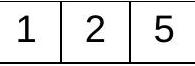
\includegraphics[max width=\textwidth]{2025_02_07_36131546116d12814c9cg-04}
\end{center}

\section*{ZadAnia otwarte (niekodowane)}
\begin{enumerate}
  \item Akceptowane są wszystkie rozwiązania merytorycznie poprawne i spełniające warunki zadania.
  \item Jeżeli zdający popełni błędy rachunkowe, które na żadnym etapie rozwiązania nie upraszczają inie zmieniają danego zagadnienia, lecz stosuje poprawną metodę i konsekwentnie do popełnionych błędów rachunkowych rozwiązuje zadanie, to może otrzymać co najwyżej ( $n-1$ ) punktów (gdzie $n$ jest maksymalną możliwą do uzyskania liczbą punktów za dane zadanie).
\end{enumerate}

Zadanie 6. (0-3)

\begin{center}
\begin{tabular}{|c|l|}
\hline
\multicolumn{2}{|c|}{Wymagania egzaminacyjne 2021} \\
\hline
\multicolumn{1}{|c|}{Wymaganie ogólne} & \multicolumn{1}{c|}{Wymaganie szczegółowe} \\
\hline
V. Rozumowanie i argumentacja. & Zdajacy: \\
 & R1.2) stosuje w obliczeniach wzór na \\
 & logarytm potęgi oraz wzór na zamianę \\
 & podstawy logarytmu. \\
\hline
\end{tabular}
\end{center}

\section*{Zasady oceniania}
\section*{Zdający otrzymuje}
 1 p. gdy podczas przekształcenia wyrażenia $\log _{3} 4$ lub $\frac{4}{\log _{2} 18-1}$ poprawnie zastosuje wzór na zamianę podstaw logarytmu lub logarytm ilorazu/iloczynu, lub logarytm potęgi, np.:$$
\log _{3} 4=\frac{\log _{2} 4}{\log _{2} 3}, \frac{4}{\log _{2} 18-1}=\frac{4}{\log _{2} \frac{18}{2}}, \quad \log _{3} 4=2 \log _{3} 2, \log _{2} 18=\log _{2} 2+\log _{2} 9
$$

Zdający otrzymuje 2 p. gdy:

\begin{itemize}
  \item przekształci wyrażenie $\log _{3} 4$ lub $\frac{4}{\log _{2} 18-1}$ lub oba te wyrażenia do takiej postaci, z której poprzez jednokrotne zastosowanie wzoru na zamianę podstaw logarytmu lub logarytm ilorazu/iloczynu, lub logarytm potęgi oraz ewentualne kilkukrotne przekształcenie wyrażenia wymiernego uzyskuje się tezę
\end{itemize}

\section*{ALBO}
\begin{itemize}
  \item wyznaczy $\log _{2} 3 \mathrm{w}$ zależności od $c: \log _{2} 3=\frac{c-1}{2}$
\end{itemize}

\section*{Zdający otrzymuje \\
 3 p. \\
 gdy, stosując poprawną metodę, przeprowadzi pełny dowód.}
\section*{Uwaga:}
Jeżeli zdający, przy rozpoczęciu przekształcania wyrażenia $\log _{3} 4$ lub $\frac{4}{\log _{2} 18-1}$, popełnia błąd rzeczowy (niepoprawnie zastosuje wzór na zamianę podstaw logarytmu lub logarytm ilorazu/iloczynu, lub logarytm potęgi), lecz w dalszej części rozwiązania każdorazowo stosuje te wzory poprawnie, to może otrzymać za całe rozwiązanie co najwyżej 1 punkt.

\section*{Przykładowe pełne rozwiązania}
\section*{Sposób 1.}
Przekształcamy wyrażenie $\log _{3} 4$, stosując wzór na zamianę podstawy logarytmu:

$$
\log _{3} 4=\frac{\log _{2} 4}{\log _{2} 3}
$$

Aby doprowadzić do uzyskania w liczniku liczby 4, mnożymy licznik i mianownik ułamka przez 2. Otrzymujemy:

$$
\frac{2 \cdot \log _{2} 4}{2 \cdot \log _{2} 3}=\frac{2 \cdot \log _{2} 4}{\log _{2} 9}=\frac{4}{\log _{2} 9}
$$

Stosujemy wzór na różnicę logarytmów o tych samych podstawach i otrzymujemy:

$$
\frac{4}{\log _{2} 9}=\frac{4}{\log _{2} \frac{18}{2}}=\frac{4}{\log _{2} 18-\log _{2} 2}=\frac{4}{c-1}
$$

Zatem $\log _{3} 4=\frac{4}{c-1}$. To należało wykazać.

\section*{Sposób 2.}
Podstawiamy $\log _{2} 18=c$ do wyrażenia $\frac{4}{c-1}$ i zapisujemy mianownik jako różnicę logarytmów o podstawie 2 :

$$
\frac{4}{c-1}=\frac{4}{\log _{2} 18-\log _{2} 2}
$$

Przekształcamy wyrażenie w mianowniku:

$$
\frac{4}{\log _{2} 18-\log _{2} 2}=\frac{4}{\log _{2} 9}=\frac{4}{2 \log _{2} 3}=\frac{2}{\log _{2} 3}
$$

Stosujemy wzór na zamianę podstawy logarytmu:

$$
\frac{2}{\log _{2} 3}=\frac{2}{\frac{1}{\log _{3} 2}}=2 \log _{3} 2=\log _{3} 4
$$

Zatem $\frac{4}{c-1}=\log _{3} 4$. To należało wykazać.

\section*{Sposób 3.}
Przekształcamy $\log _{2} 18=\log _{2}(9 \cdot 2)=\log _{2} 9+\log _{2} 2=\log _{2} 9+1=2 \log _{2} 3+1=c$\\
Obliczamy $\log _{2} 3=\frac{c-1}{2}$. Stąd

$$
\log _{3} 4=\frac{\log _{2} 4}{\log _{2} 3}=\frac{2}{\frac{c-1}{2}}=\frac{4}{c-1}
$$

To należało wykazać.

\section*{Zadanie 7. (0-3)}
\begin{center}
\begin{tabular}{|l|l|}
\hline
\multicolumn{2}{|c|}{Wymagania egzaminacyjne 2021} \\
\hline
\multicolumn{1}{|c|}{Wymaganie ogólne} & \multicolumn{1}{c|}{Wymaganie szczegółowe} \\
\hline
\begin{tabular}{ll}
II. Wykorzystanie i interpretowanie &  \\
reprezentacji. & Zdajacy: \\
 & R3.7) rozwiązuje proste nierówności \\
 & wymierne [...]. \\
\hline
\end{tabular} &  \\
\hline
\end{tabular}
\end{center}

\section*{Zasady oceniania}
Zdający otrzymuje\\
gdy:

\begin{itemize}
  \item przekształci nierówność $\frac{2 x-1}{1-x} \leq \frac{2+2 x}{5 x}$ do postaci $\frac{12 x^{2}-5 x-2}{(1-x) \cdot 5 x} \leq 0 \quad$ lub $\frac{(2 x-1) \cdot 5 x-(2+2 x)(1-x)}{(1-x) \cdot 5 x} \leq 0$\\
ALBO
  \item przekształci nierówność $\frac{2 x-1}{1-x} \leq \frac{2+2 x}{5 x}$, mnożąc obie strony tej nierówności przez iloczyn $(1-x)^{2}(5 x)^{2}$, do postaci
\end{itemize}

$$
5 x \cdot(1-x)[(2 x-1) \cdot 5 x-(2+2 x) \cdot(1-x)] \leq 0, \text { gdzie } x \neq 0 \text { i } x \neq 1
$$

ALBO

\begin{itemize}
  \item przyjmie, że $x \in(-\infty, 0) \cup(1,+\infty)$ i przekształci nierówność $\frac{2 x-1}{1-x} \leq \frac{2+2 x}{5 x}$ $\{m n o z ̇ a ̨ c ~ o b i e ~ s t r o n y ~ n i e r o ́ w n o s ́ c i ~ p r z e z ~ i l o c z y n ~(1-x) 5 x\} ~ d o ~ p o s t a c i ~ i$
\end{itemize}

$$
(2 x-1) \cdot 5 x \geq(2+2 x)(1-x)
$$

\section*{ALBO}
\begin{itemize}
  \item przyjmie, że $x \in(0,1)$ i przekształci nierówność $\frac{2 x-1}{1-x} \leq \frac{2+2 x}{5 x}$ \{mnożąc obie strony nierówności przez iloczyn $(1-x) 5 x$ \} do postaci
\end{itemize}

$$
(2 x-1) \cdot 5 x \leq(2+2 x)(1-x)
$$

Zdający otrzymuje\\
2p. gdy:

\begin{itemize}
  \item przekształci nierówność $\frac{12 x^{2}-5 x-2}{(1-x) \cdot 5 x} \leq 0$ lub $5 x \cdot(1-x)[(2 x-1) \cdot 5 x-(2+2 x) \cdot(1-x)] \leq 0$ do postaci iloczynowej i zapisze
\end{itemize}

$$
12\left(x-\frac{2}{3}\right)\left(x+\frac{1}{4}\right)(1-x) \cdot 5 x \leq 0, \text { gdzie } x \neq 0 \text { i } x \neq 1
$$

ALBO

\begin{itemize}
  \item rozwiąże nierówność $(2 x-1) 5 x \geq(2+2 x)(1-x)$ dla $x \in(-\infty, 0) \cup(1,+\infty)$ i zapisze:
\end{itemize}

$$
x \in\left(-\infty,-\frac{1}{4}\right\rangle \cup(1,+\infty)
$$

ALBO

\begin{itemize}
  \item rozwiąże nierówność $(2 x-1) 5 x \leq(2+2 x)(1-x)$ dla $x \in(0,1)$ i zapisze:
\end{itemize}

$$
x \in\left(0, \frac{2}{3}\right)
$$

ALBO

\begin{itemize}
  \item spełni wymagania za 1 punkt oraz obliczy wszystkie pierwiastki wielomianów $12 x^{2}-5 x-2$ i $5 x(1-x)$ \{albo wielomianów $5 x(2 x-1)$ i $\left.(2+2 x)(1-x)\right\}$
\end{itemize}

\section*{Zdający otrzymuje}
3p.\\
gdy zastosuje poprawną metodę rozwiązania nierówności i otrzyma poprawny wynik:

$$
x \in\left(-\infty,-\frac{1}{4}\right\rangle \cup\left(0, \frac{2}{3}\right\rangle \cup(1,+\infty) .
$$

\section*{Uwagi:}
\begin{enumerate}
  \item Jeśli zdający mnoży obie strony nierówności przez iloczyn mianowników bez rozpatrzenia znaków tego iloczynu, to otrzymuje 0 punktów za całe rozwiązanie.
  \item Jeśli zdający nie wyłączy ze zbioru rozwiązań nierówności liczb $x=0$ i $x=1$, to otrzymuje za całe rozwiązanie co najwyżej 2 punkty.
\end{enumerate}

\section*{Przykładowe pełne rozwiązania}
\section*{Sposób 1.}
Zakładamy, że $x \neq 0$ i $x \neq 1$. Przekształcamy równoważnie podaną nierówność:

$$
\frac{2 x-1}{1-x}-\frac{2+2 x}{5 x} \leq 0
$$

$$
\begin{gathered}
\frac{10 x^{2}-5 x-2-2 x+2 x+2 x^{2}}{5 x(1-x)} \leq 0 \\
\frac{12 x^{2}-5 x-2}{5 x(1-x)} \leq 0
\end{gathered}
$$

Stąd dostajemy

$$
12\left(x-\frac{2}{3}\right)\left(x+\frac{1}{4}\right)(1-x) \cdot 5 x \leq 0 \text { i } x \neq 0 \text { i } x \neq 1
$$

Zatem $x \in\left(-\infty,-\frac{1}{4}\right) \cup\left(0, \frac{2}{3}\right) \cup(1,+\infty)$.

\section*{Sposób 2.}
Zakładamy, że $x \neq 0$ i $x \neq 1$. Przekształcamy równoważnie podaną nierówność:

$$
\begin{gathered}
\frac{2 x-1}{1-x}-\frac{2+2 x}{5 x} \leq 0 / \cdot(1-x)^{2}(5 x)^{2} \\
5 x(1-x)\left[10 x^{2}-5 x-\left(2+2 x-2 x-2 x^{2}\right)\right] \leq 0, \\
5 x(1-x)\left[10 x^{2}-5 x-2+2 x^{2}\right] \leq 0, \\
12(1-x)\left(x+\frac{1}{4}\right)\left(x-\frac{2}{3}\right) 5 x \leq 0 \text { i } x \neq 0 \text { i } x \neq 1 .
\end{gathered}
$$

Zatem $x \in\left(-\infty,-\frac{1}{4}\right) \cup\left(0, \frac{2}{3}\right) \cup(1,+\infty)$.

\section*{Sposób 3.}
\begin{enumerate}
  \item Rozwiązujemy nierówność $\frac{2 x-1}{1-x} \leq \frac{2+2 x}{5 x}$ w zbiorze $(-\infty, 0) \cup(1,+\infty)$.
\end{enumerate}

Przekształcamy równoważnie podaną nierówność:

$$
\begin{gathered}
\frac{2 x-1}{1-x}-\frac{2+2 x}{5 x} \leq 0 \quad / \cdot(1-x) 5 x \\
(2 x-1) 5 x \geq(2+2 x)(1-x) \\
12 x^{2}-5 x-2 \geq 0
\end{gathered}
$$

Otrzymujemy $x_{1}=-\frac{1}{4}, x_{2}=\frac{2}{3}$ oraz $x \in\left(-\infty,-\frac{1}{4}\right) \cup(1,+\infty)$.\\
2. Rozwiązujemy nierówność $\frac{2 x-1}{1-x} \leq \frac{2+2 x}{5 x}$ w zbiorze $(0,1)$.

Przekształcamy równoważnie podaną nierówność:

$$
\begin{gathered}
\frac{2 x-1}{1-x}-\frac{2+2 x}{5 x} \leq 0 \quad / \cdot(1-x) 5 x \\
(2 x-1) 5 x \leq(2+2 x)(1-x) \\
12 x^{2}-5 x-2 \leq 0
\end{gathered}
$$

Otrzymujemy $x_{1}=-\frac{1}{4}, x_{2}=\frac{2}{3}$ oraz $x \in\left(0, \frac{2}{3}\right)$.\\
Zatem zbiorem rozwiązań nierówności $\frac{2 x-1}{1-x} \leq \frac{2+2 x}{5 x}$ jest $\left(-\infty,-\frac{1}{4}\right) \cup\left(0, \frac{2}{3}\right) \cup(1,+\infty)$.

Zadanie 8. (0-3)

\begin{center}
\begin{tabular}{|l|l|}
\hline
\multicolumn{2}{|c|}{Wymagania egzaminacyjne 2021} \\
\hline
\multicolumn{1}{|c|}{Wymaganie ogólne} & \multicolumn{1}{|c|}{Wymagania szczegółowe} \\
\hline
V. Rozumowanie i argumentacja & Zdający: \\
 & G10.13) stosuje cechy przystawania \\
 & trójkątów [...]. \\
 & R7.3) rozpoznaje figury podobne [...]. \\
\hline
\end{tabular}
\end{center}

\section*{Zasady oceniania}
\section*{Zdający otrzymuje}
gdy:

\begin{itemize}
  \item zapisze, że trójkąty $A B E$ i $B C D$ (lub $E B C$ i $D C A$ ) są przystające
\end{itemize}

ALBO

\begin{itemize}
  \item zapisze, że trójkąty $D B P$ i $D C B$ (lub $E B A$ ) są podobne lub zapisze odpowiednie proporcje wynikające $z$ tego podobieństwa\\
ALBO
  \item wyznaczy długość odcinka $C D$ w zależności od $|D B|:|C D|=|D B| \cdot \sqrt{7}$
\end{itemize}

ALBO

\begin{itemize}
  \item zastosuje twierdzenie o stosunku pól trójkątów o tych samych wysokościach (np. w sposobie 8. zapisze, że $\frac{P_{F D P}}{P_{D G P}}=\frac{|F D|}{|D G|}$ )\\
ALBO
  \item umieści trójkąt $A B C$ w układzie współrzędnych i wyznaczy współrzędne punktów $D$ i $E$ w zależności od długości boku trójkąta $A B C$\\
ALBO
  \item narysuje odcinek $D F$ równoległy do $A C$ (sposób 5.) i zapisze, że trójkąty $D G P$ i $C E P$ (lub trójkąty $D B G$ i $A B E$ ) są podobne\\
ALBO
  \item narysuje odcinek $G F$ równoległy do $A C$ (sposób 7.) i zapisze, że trójkąty $G D P$ i $A D C$ (lub trójkąty $G B P$ i $A B E$ ) są podobne\\
ALBO
  \item narysuje odcinek $E F$ równoległy do $A B$ (sposób 4.) i zapisze, że trójkąty $A D C$ i $E G C$ (lub $D B C$ i $G F C$, lub trójkąty $D B P$ i $G E P$ ) są podobne\\
ALBO
  \item zapisze, że trójkąty $D B P$ i $D A F$ są podobne (sposób 10.) lub zapisze odpowiednie proporcje wynikające $z$ tego podobieństwa\\
Zdający otrzymuje
  \item zapisze, że trójkąty $D B P$ i $D C B$ (lub $E B A$ ) są podobne i obliczy skalę ich podobieństwa: $s=\frac{1}{\sqrt{7}}$\\
ALBO
  \item zapisze układ nie więcej niż czterech niezależnych równań liniowych prowadzących do uzasadnienia tezy\\
ALBO
  \item zapisze równanie z dwiema niewiadomymi $m$ i $a$, np.\\
$\left(\frac{1}{3} a\right)^{2}=m^{2}+(3 m)^{2}-2 \cdot m \cdot 3 m \cdot \frac{1}{2} \quad$ (sposób 3.) oraz zapisze, że pole trójkąta $D B P$ jest równe $P_{D B P}=\frac{1}{2} \cdot|D P| \cdot|B P| \cdot \sin 60^{\circ}$\\
ALBO
  \item wyznaczy stosunek długości odcinka $D P$ do długości odcinka $C D: \frac{|D P|}{|C D|}=\frac{1}{7}$ (sposoby 4., 5., 6. i 7.)
\end{itemize}

ALBO

\begin{itemize}
  \item zapisze w zależności od $x=P_{D G P}$ pola trójkątów: $F G P, P H K, M P L, D B P$ i co najmniej jednego z trójkątów $A F P$ (lub $A P M$ ), $P K C$ (lub $P C L$ ): $P_{F G P}=3 x$, $P_{P H K}=12 x, P_{M P L}=48 x, P_{D B P}=7 x, P_{P F P}=6 x, P_{P K C}=24 x$ (sposób 8.)\\
ALBO
  \item obliczy drugą współrzędną punktu $P$ w zależności od przyjętej zmiennej: $y_{P}=\frac{\sqrt{3}}{14} a$ (sposób 9.)\\
ALBO
  \item zapisze $P_{D B P}=\frac{1}{3} P_{P F B}$ i $P_{A B C}=P_{P R S}+P_{A B S}+P_{B C P}+P_{C A R}$ (sposób 10.)
\end{itemize}

\section*{Zdający otrzymuje}
3 p.\\
gdy przeprowadzi pełne rozumowanie.

\section*{Przykładowe pełne rozwiązania}
\section*{Sposób 1.}
Trójkąty $A B E$ i $B C D$ są przystające, gdyż $|A B|=|B C|,|\Varangle B A E|=|\Varangle C B D|=60^{\circ}$ oraz $|A E|=|B D|$. Zatem $|\Varangle A B E|=|\Varangle B C D|$ oraz $|\Varangle A E B|=|\Varangle B D C|$. Stąd wynika (cecha KKK), że trójkąt $D B P$ jest podobny do trójkąta $D C B$, a skala tego podobieństwa jest równa

$$
s=\frac{|B D|}{|C D|} .
$$

Niech $|D B|=a$. Wtedy $|B C|=3 a$. Z twierdzenia cosinusów dla trójkąta $D B C$ otrzymujemy

$$
|C D|=\sqrt{|B D|^{2}+|B C|^{2}-2 \cdot|B D| \cdot|B C| \cdot \cos 60^{\circ}}=\sqrt{a^{2}+(3 a)^{2}-2 \cdot a \cdot 3 a \cdot \frac{1}{2}}=\sqrt{7} a
$$

Zatem $s=\frac{a}{a \sqrt{7}}=\frac{1}{\sqrt{7}}$.\\
Pole trójkąta $D B C$ jest trzecią częścią pola trójkąta $A B C$, gdyż oba te trójkąty mają wspólną wysokość opuszczoną z wierzchołka $C$ oraz $|B D|=\frac{1}{3}|A B|$.\\
Ponieważ stosunek pól figur podobnych jest równy kwadratowi skali ich podobieństwa, więc

$$
P_{\triangle D B P}=s^{2} \cdot P_{\triangle D B C}=\left(\frac{1}{\sqrt{7}}\right)^{2} \cdot \frac{1}{3} \cdot P_{\triangle A B C}=\frac{1}{21} \cdot P_{\triangle A B C}
$$

To należało wykazać.

\section*{Uwagi:}
\begin{enumerate}
  \item Po wyznaczeniu długości $|C D|=|B E|$ można wyznaczyć sinus kąta $D B E$, korzystając z twierdzenia sinusów. Wtedy otrzymujemy
\end{enumerate}

$$
\frac{|B E|}{\frac{\sqrt{3}}{2}}=\frac{a}{\sin |\Varangle D B E|}
$$

skąd $\sin |\Varangle D B E|=\frac{\sqrt{3}}{2 \sqrt{7}}$, więc

$$
P_{\triangle D B P}=\frac{1}{2} \cdot a \cdot\left(\frac{1}{\sqrt{7}} \cdot 3 a\right) \cdot \frac{\sqrt{3}}{2 \sqrt{7}}=\frac{3 a^{2} \sqrt{3}}{28}=\frac{(3 a)^{2} \sqrt{3}}{4} \cdot \frac{1}{21}=\frac{1}{21} \cdot P_{\triangle A B C}
$$

\begin{enumerate}
  \setcounter{enumi}{1}
  \item Długość odcinka $C D$ możemy też obliczyć w inny sposób. Poniżej przedstawiamy dwa z tych sposobów:\\
a) Niech $M$ oznacza spodek wysokości trójkąta $A B C$ opuszczonej z wierzchołka $C$. Wtedy
\end{enumerate}

$$
|C M|=\frac{3 a \sqrt{3}}{2} \text { oraz }|M D|=|M B|-|D B|=\frac{1}{2} \cdot 3 a-a=\frac{1}{2} a
$$

Z twierdzenia Pitagorasa dla trójkąta MDC otrzymujemy

$$
|C D|=\sqrt{\left(\frac{1}{2} a\right)^{2}+\left(\frac{3 a \sqrt{3}}{2}\right)^{2}}=\sqrt{\frac{28}{4} a^{2}}=a \sqrt{7}
$$

b) Z twierdzenia Stewarta otrzymujemy

$$
\begin{gathered}
(3 a)^{2} \cdot 2 a+(3 a)^{2} \cdot a=3 a \cdot\left(|C D|^{2}+2 a \cdot a\right) \\
3 a \cdot 2 a+3 a \cdot a=|C D|^{2}+2 a^{2} \\
|C D|^{2}=7 a^{2} \\
|C D|=a \sqrt{7}
\end{gathered}
$$

Sposób 2.\\
Przyjmijmy, że $P_{\triangle A B C}=S, P_{\triangle D B P}=Q, P_{\triangle A P E}=Y, P_{\triangle B C P}=X$.\\
W dalszym ciągu rozumowania będziemy wielokrotnie korzystać z faktu, że stosunek pól trójkątów o wspólnej wysokości jest równy stosunkowi długości podstaw, na które ta wysokość jest opuszczona.\\
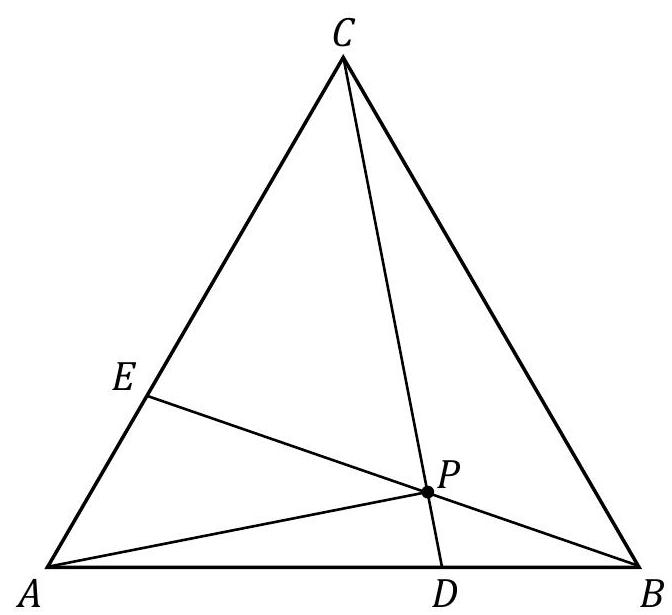
\includegraphics[max width=\textwidth, center]{2025_02_07_36131546116d12814c9cg-12}

Zatem $P_{A B E}=\frac{1}{3} S, P_{C B E}=\frac{2}{3} S, P_{D B C}=\frac{1}{3} S, P_{A D C}=\frac{2}{3} S$. Ponadto

$$
\frac{P_{A P E}}{P_{C P E}}=\frac{1}{2} \quad \text { oraz } \frac{P_{D B P}}{P_{A D P}}=\frac{1}{2}
$$

Otrzymaliśmy więc układ równań

$$
\left\{\begin{array}{l}
Q+X=\frac{1}{3} S \\
2 Y+X=\frac{2}{3} S \\
Y+3 Q=\frac{1}{3} S
\end{array}\right.
$$

Wyznaczając wielkość $X$ z pierwszego równania i wielkość $Y$ z trzeciego oraz wstawiając wyznaczone wielkości do równania drugiego, otrzymujemy:

$$
\begin{gathered}
2\left(\frac{1}{3} S-3 Q\right)+\left(\frac{1}{3} S-Q\right)=\frac{2}{3} S \\
\frac{1}{3} S=7 Q \\
Q=\frac{1}{21} S
\end{gathered}
$$

To należało wykazać.\\
Sposób 3.\\
Trójkąty $A B E$ i $B C D$ są przystające, gdyż $|A B|=|B C|,|\Varangle B A E|=|\Varangle C B D|=60^{\circ}$ oraz $|A E|=|B D|$. Zatem $|\Varangle A B E|=|\Varangle B C D|$ oraz $|\Varangle A E B|=|\Varangle B D C|$. Stąd wynika (cecha KKK), że trójkąt $D B P$ jest podobny do trójkąta $D C B$.\\
Zatem $\frac{|A E|}{|A B|}=\frac{|D P|}{|B P|}=\frac{1}{3}$, więc $|B P|=3|D P|$ oraz $|\Varangle B P D|=60^{\circ}$. Oznaczmy $|D P|=m$.\\
Wtedy $|B P|=3 \mathrm{~m}$.\\
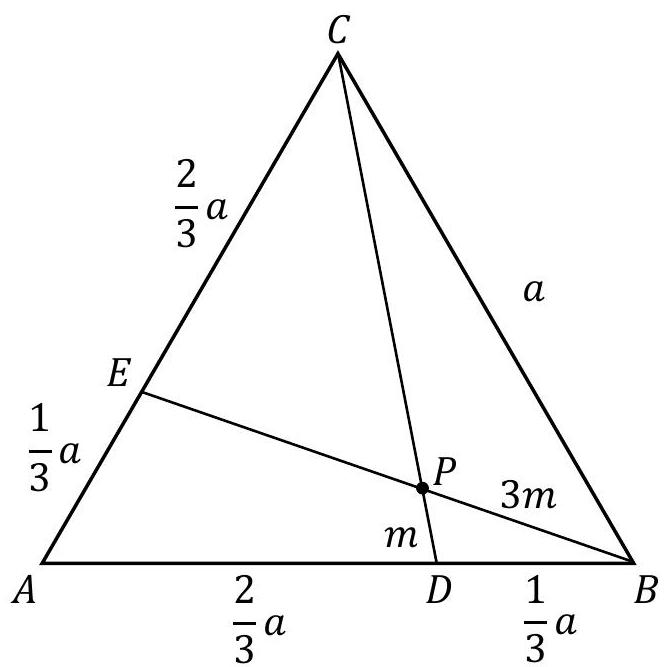
\includegraphics[max width=\textwidth, center]{2025_02_07_36131546116d12814c9cg-13}

Z twierdzenia cosinusów dla trójkąta $D B P$ otrzymujemy

$$
|B D|^{2}=|D P|^{2}+|B P|^{2}-2 \cdot|D P| \cdot|B P| \cdot \cos 60^{\circ}
$$

czyli

$$
\left(\frac{1}{3} a\right)^{2}=m^{2}+(3 m)^{2}-2 \cdot m \cdot 3 m \cdot \frac{1}{2}
$$

Stąd

$$
\begin{aligned}
& \frac{1}{9} a^{2}=7 m^{2} \\
& m^{2}=\frac{1}{63} a^{2}
\end{aligned}
$$

Pole trójkąta $D B P$ jest równe

$$
\begin{aligned}
P_{D B P} & =\frac{1}{2} \cdot|D P| \cdot|B P| \cdot \sin 60^{\circ}=\frac{1}{2} \cdot m \cdot 3 m \cdot \frac{\sqrt{3}}{2}=\frac{3}{4} \cdot m^{2} \sqrt{3}= \\
& =\frac{3}{4} \cdot \frac{1}{63} a^{2} \sqrt{3}=\frac{1}{21} \cdot \frac{a^{2} \sqrt{3}}{4}=\frac{1}{21} \cdot P_{A B C}
\end{aligned}
$$

To należało wykazać.

\section*{Sposób 4.}
Oznaczmy przez a długość boku trójkąta $A B C$. Prowadzimy odcinek $E F$ równoległy do boku $A B$ trójkąta $A B C$.\\
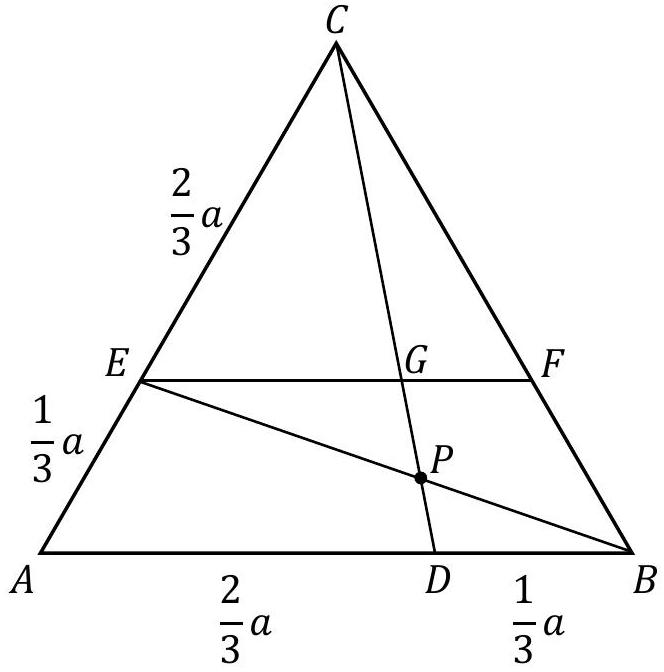
\includegraphics[max width=\textwidth, center]{2025_02_07_36131546116d12814c9cg-14}

Trójkąty $A D C$ i $E G C$ są podobne (cecha KKK), więc

$$
\frac{|E G|}{|C E|}=\frac{|A D|}{|A C|}=\frac{2}{3} \text { oraz } \frac{|C G|}{|C D|}=\frac{|C E|}{|A C|}=\frac{2}{3}
$$

Stąd

$$
|E G|=\frac{2}{3}|C E|=\frac{2}{3} \cdot \frac{2}{3} a=\frac{4}{9} a \text { oraz }|C G|=\frac{2}{3}|C D|
$$

$Z$ drugiej równości wynika, że $|G D|=\frac{1}{3}|C D|$.\\
Trójkąty $D B P$ i $G E P$ są podobne (cecha KKK), więc

$$
\frac{|D P|}{|G P|}=\frac{|D B|}{|E G|}=\frac{\frac{1}{3} a}{\frac{4}{9} a}=\frac{3}{4}
$$

Zatem

$$
|D P|=\frac{3}{7}|D G|=\frac{3}{7} \cdot \frac{1}{3}|C D|=\frac{1}{7}|C D|
$$

Trójkąty $D B P$ i $D B C$ mają wspólną wysokość opuszczoną z wierzchołka $B$, więc

$$
\frac{P_{D B P}}{P_{D B C}}=\frac{|D P|}{|D C|}=\frac{1}{7}, \quad \text { czyli } \quad P_{D B P}=\frac{1}{7} P_{D B C} .
$$

Ponadto $P_{D B C}=\frac{1}{3} P_{A B C}$, gdyż trójkąty $D B C$ i $A B C$ mają wspólną wysokość opuszczoną z wierzchołka $C$ i $|D B|=\frac{1}{3}|A B|$, więc

$$
P_{D B P}=\frac{1}{7} P_{D B C}=\frac{1}{7} \cdot \frac{1}{3} P_{A B C}=\frac{1}{21} P_{A B C} .
$$

To należało wykazać.

\section*{Sposób 5.}
Oznaczmy przez a długość boku trójkąta $A B C$. Prowadzimy odcinek $D F$ równoległy do boku $A C$ trójkąta $A B C$. Niech $G$ oznacza punkt przecięcia odcinków $B E$ i $D F$.\\
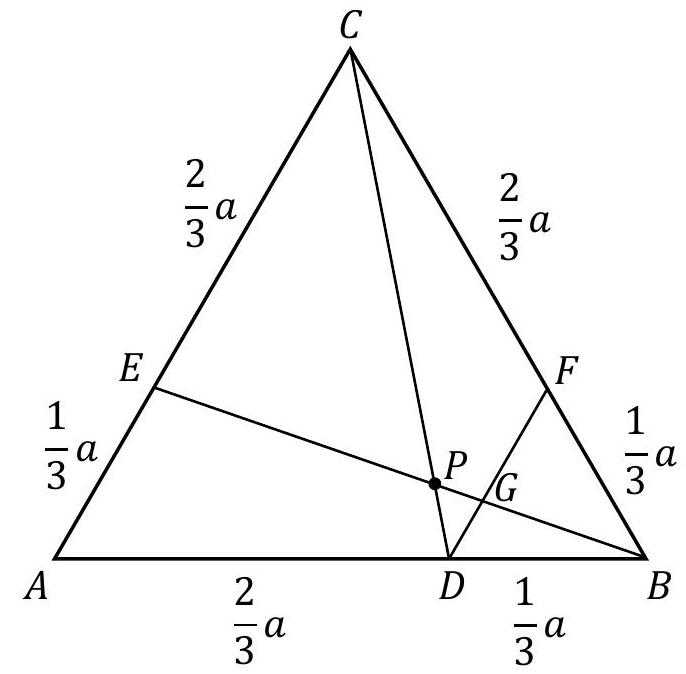
\includegraphics[max width=\textwidth, center]{2025_02_07_36131546116d12814c9cg-15}

Trójkąt $D B F$ jest równoboczny, a jego bok ma długość $\frac{1}{3} a$.\\
Trójkąty $D B G$ i $A B E$ są podobne (cecha KKK), więc

$$
\frac{|D G|}{|D B|}=\frac{|A E|}{|A B|}=\frac{1}{3}
$$

Stąd

$$
|D G|=\frac{1}{3} \cdot \frac{1}{3} a=\frac{1}{9} a
$$

Trójkąty $D G P$ i $C E P$ są podobne (cecha KKK), więc

$$
\frac{|D P|}{|C P|}=\frac{|D G|}{|C E|}=\frac{\frac{1}{9} a}{\frac{2}{3} a}=\frac{1}{6}
$$

Zatem $|D P|=\frac{1}{7}|C D|$.\\
Trójkąty $D B P$ i $D B C$ mają wspólną wysokość opuszczoną z wierzchołka $B$, więc

$$
\frac{P_{D B P}}{P_{D B C}}=\frac{|D P|}{|D C|}=\frac{1}{7}, \quad \text { czyli } \quad P_{D B P}=\frac{1}{7} P_{D B C} .
$$

Ponadto $P_{D B C}=\frac{1}{3} P_{A B C}$, gdyż trójkąty $D B C$ i $A B C$ mają wspólną wysokość opuszczoną z wierzchołka $C$ i $|D B|=\frac{1}{3}|A B|$, więc

$$
P_{D B P}=\frac{1}{7} P_{D B C}=\frac{1}{7} \cdot \frac{1}{3} P_{A B C}=\frac{1}{21} P_{A B C} .
$$

To należało wykazać.

\section*{Sposób 6.}
Oznaczmy przez $a$ długość boku trójkąta $A B C$. Wtedy $|A D|=|C E|=\frac{2}{3} a$ oraz $|A E|=|D B|=\frac{1}{3} a$. Prowadzimy odcinek $E F$ równoległy do boku $C D$ trójkąta $A C D$.\\
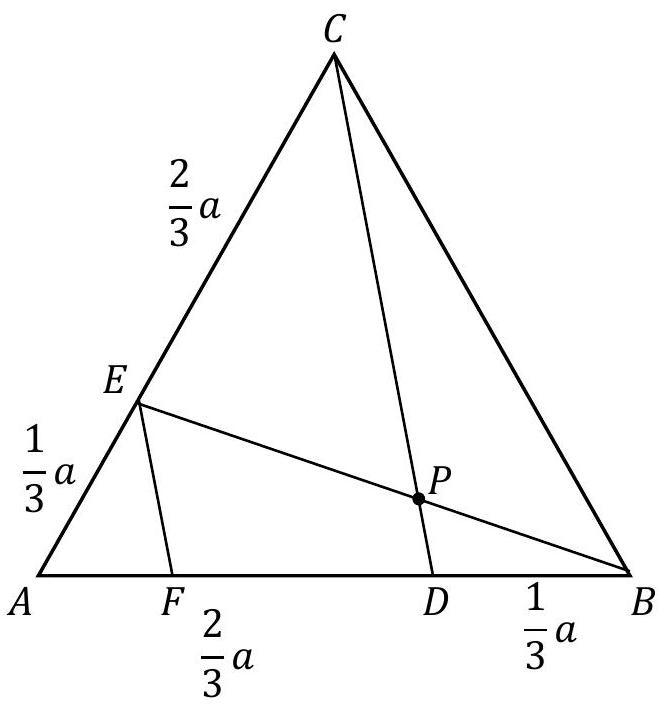
\includegraphics[max width=\textwidth, center]{2025_02_07_36131546116d12814c9cg-16}

Trójkąty $A F E$ i $A D C$ są podobne (cecha KKK), więc

$$
\frac{|E F|}{|C D|}=\frac{|A E|}{|A C|}=\frac{1}{3} \text { oraz } \frac{|A F|}{|A E|}=\frac{|A D|}{|A C|}=\frac{2}{3}
$$

Stąd

$$
|E F|=\frac{1}{3}|C D| \text { oraz }|A F|=\frac{2}{3}|A E|=\frac{2}{3} \cdot \frac{1}{3} a=\frac{2}{9} a
$$

Zatem $|F B|=|A B|-|A F|=a-\frac{2}{9} a=\frac{7}{9} a$.\\
Trójkąty $F B E$ i $D B P$ są podobne (cecha KKK), więc

$$
\frac{|P D|}{|E F|}=\frac{|D B|}{|F B|}=\frac{\frac{1}{3} a}{\frac{7}{9} a}=\frac{3}{7}
$$

Stąd

$$
|D P|=\frac{3}{7}|E F|=\frac{3}{7} \cdot \frac{1}{3}|C D|=\frac{1}{7}|C D|
$$

Trójkąty $D B P$ i $D B C$ mają wspólną wysokość opuszczoną z wierzchołka $B$, więc

$$
\frac{P_{D B P}}{P_{D B C}}=\frac{|D P|}{|D C|}=\frac{1}{7}, \quad \text { czyli } \quad P_{D B P}=\frac{1}{7} P_{D B C} .
$$

Ponadto $P_{D B C}=\frac{1}{3} P_{A B C}$, gdyż trójkąty $D B C$ i $A B C$ mają wspólną wysokość opuszczoną z wierzchołka $C$ i $|D B|=\frac{1}{3}|A B|$, więc

$$
P_{D B P}=\frac{1}{7} P_{D B C}=\frac{1}{7} \cdot \frac{1}{3} P_{A B C}=\frac{1}{21} P_{A B C} .
$$

To należało wykazać.

\section*{Sposób 7.}
Przez punkt $P$ prowadzimy odcinek $G F$ równoległy do boku $A C$ trójkąta $A B C$. Trójkąt $G F B$ jest równoboczny. Oznaczmy długość boku trójkąta $A B C$ przez a i odcinka $B F$ przez $x$.\\
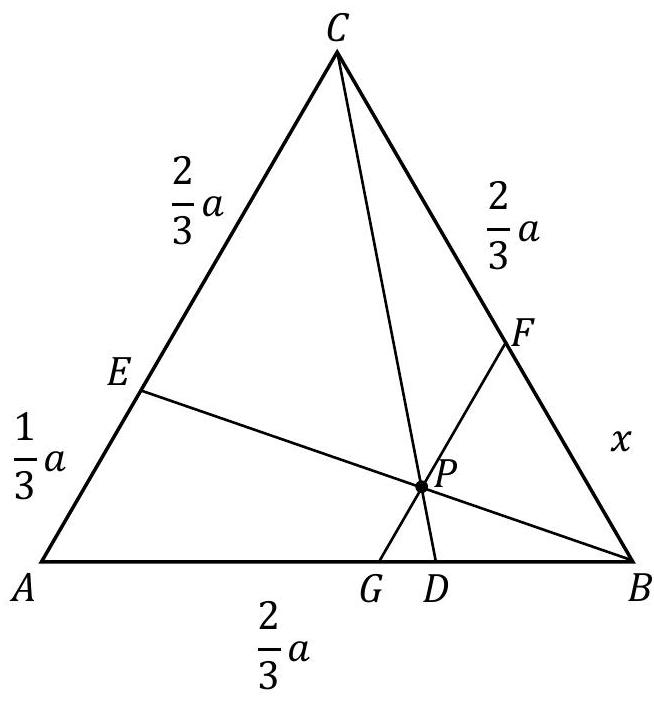
\includegraphics[max width=\textwidth, center]{2025_02_07_36131546116d12814c9cg-17}

Trójkąty $G B P$ i $A B E$ są podobne (cecha KKK), więc

$$
\frac{|G P|}{|G B|}=\frac{|A E|}{|A B|}=\frac{\frac{1}{3} a}{a}=\frac{1}{3}
$$

Stąd $|G P|=\frac{1}{3} x$.\\
Trójkąty $G D P$ i $A D C$ są podobne (cecha KKK), więc

$$
\frac{|G P|}{|G D|}=\frac{|A C|}{|A D|}=\frac{a}{\frac{2}{3} a}=\frac{3}{2} \quad \text { oraz } \quad \frac{|P D|}{|C D|}=\frac{|G P|}{|A C|}
$$

Stąd $|G D|=\frac{2}{3}|G P|$, więc

$$
|D B|=|G B|-|G D|=x-\frac{2}{3} \cdot \frac{1}{3} x=\frac{7}{9} x
$$

Zatem $\frac{1}{3} a=\frac{7}{9} x$, czyli $x=\frac{3}{7} a$.\\
Korzystając z proporcji $\frac{|P D|}{|C D|}=\frac{|G P|}{|A C|}$, otrzymujemy

$$
\frac{|P D|}{|C D|}=\frac{\frac{1}{3} x}{a}=\frac{\frac{1}{3} \cdot \frac{3}{7} a}{a}=\frac{1}{7}
$$

Trójkąty $D B P$ i $D B C$ mają wspólną wysokość opuszczoną z wierzchołka $B$, więc

$$
\frac{P_{D B P}}{P_{D B C}}=\frac{|D P|}{|D C|}=\frac{1}{7}, \quad \text { czyli } \quad P_{D B P}=\frac{1}{7} P_{D B C} .
$$

Ponadto $P_{D B C}=\frac{1}{3} P_{A B C}$, gdyż trójkąty $D B C$ i $A B C$ mają wspólną wysokość opuszczoną z wierzchołka $C$ i $|D B|=\frac{1}{3}|A B|$, więc

$$
P_{D B P}=\frac{1}{7} P_{D B C}=\frac{1}{7} \cdot \frac{1}{3} P_{A B C}=\frac{1}{21} P_{A B C} .
$$

To należało wykazać.

\section*{Sposób 8.}
Przez punkt $P$ prowadzimy odcinki $M H, G L$ i $F K$ równoległe do boków - odpowiednio $A B, B C$ i $A C$ trójkąta $A B C$. Podzieliliśmy w ten sposób trójkąt $A B C$ na trzy trójkąty równoboczne $F G P, P H K, M P L$ i trzy równoległoboki $B G P H, P K C L$ i $A F P M$. Oznaczmy pole trójkąta $D G P$ przez $x$.\\
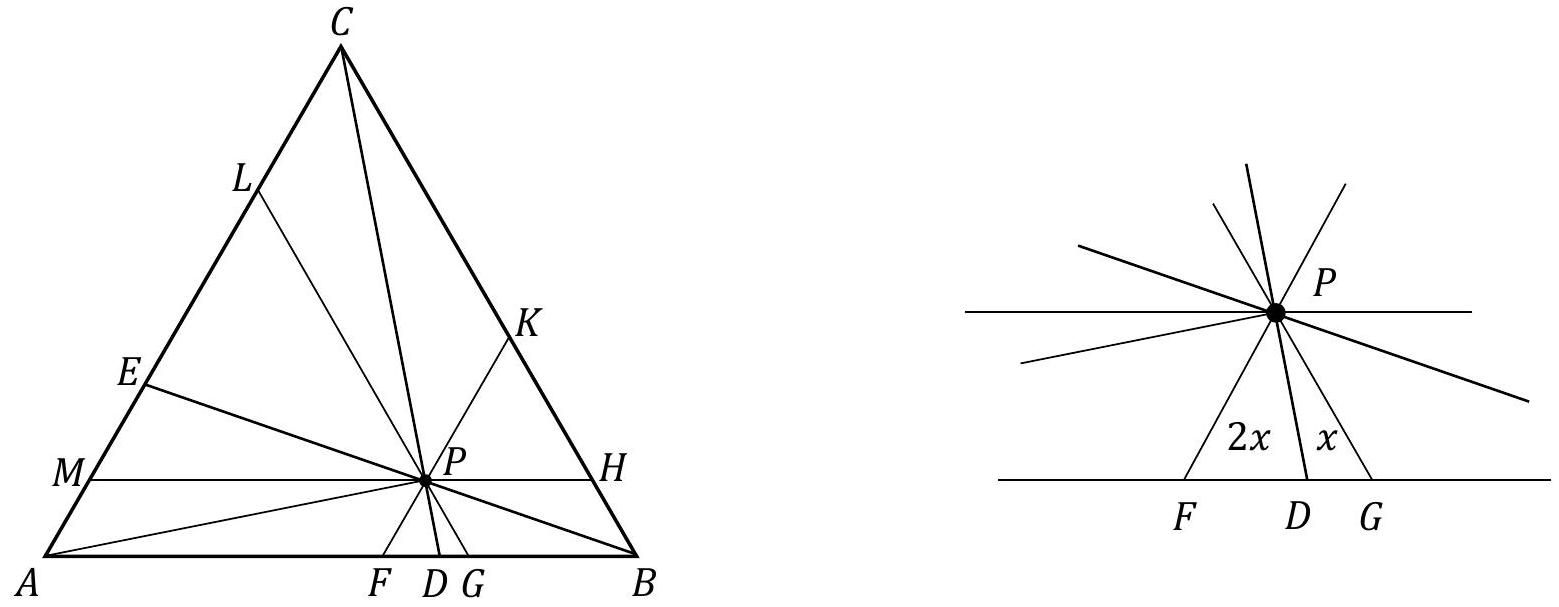
\includegraphics[max width=\textwidth, center]{2025_02_07_36131546116d12814c9cg-18}

Trójkąty $F B P$ i $A B E$ są podobne (cecha KKK). Zatem $\quad \frac{|F P|}{|F B|}=\frac{|A E|}{|A B|}=\frac{1}{3}$, więc $|F P|=\frac{1}{3}|F B|=\frac{1}{3}|F K|$, gdyż trójkąt $F B K$ jest równoboczny. Stąd $\frac{|F P|}{|P K|}=\frac{1}{2}$.\\
Tak samo wnioskujemy, że $\frac{|P H|}{|M P|}=\frac{1}{2}$.\\
Trójkąty $F D P$ i $A D C$ są podobne (cecha KKK), więc $\frac{|F P|}{|F D|}=\frac{|A C|}{|A D|}=\frac{3}{2}$, a stąd wynika, że $\frac{|D G|}{|F D|}=\frac{1}{2}$.\\
Trójkąty FDP i DGP mają wspólną wysokość opuszczoną z wierzchołka $P$, więc $\frac{P_{D G P}}{P_{F D P}}=\frac{|D G|}{|F D|}=\frac{1}{2}$, więc $P_{F D P}=2 x$, skąd $P_{F G P}=3 x$.\\
Trójkąty równoboczne są podobne, więc stosunek ich pól jest równy kwadratowi skali ich podobieństwa. Zatem

$$
\frac{P_{F G P}}{P_{P H K}}=\left(\frac{|F P|}{|P K|}\right)^{2}=\frac{1}{4}, \text { więc } P_{P H K}=4 P_{F G P}=4 \cdot 3 x=12 x
$$

oraz

$$
\frac{P_{P H K}}{P_{M P L}}=\left(\frac{|P H|}{|M P|}\right)^{2}=\frac{1}{4}, \text { więc } P_{M P L}=4 P_{P H K}=4 \cdot 12 x=48 x
$$

Trójkąty $F G P$ i $G B P$ mają wspólną wysokość opuszczoną z wierzchołka $P$, więc $\frac{P_{F G P}}{P_{G B P}}=\frac{|F G|}{|G B|}$. Trójkąty $P H K$ i $B H P$ również mają wspólną wysokość opuszczoną z wierzchołka $P$, więc $\frac{P_{P H K}}{P_{B H P}}=\frac{|K H|}{|B H|}$.\\
Zatem, wobec $|F G|=|P G|=|B H|$ oraz $|G B|=|P H|=|K H|$, otrzymujemy

$$
\frac{P_{F G P}}{P_{G B P}} \cdot \frac{P_{P H K}}{P_{B H P}}=\frac{|F G|}{|G B|} \cdot \frac{|K H|}{|B H|}=1
$$

Ponieważ $P_{G B P}=P_{B H P}$, więc $P_{G B P}=P_{B H P}=\sqrt{P_{F G P} \cdot P_{P H K}}$.\\
Analogicznie otrzymujemy $P_{K P C}=P_{P C L}=\sqrt{P_{P H K} \cdot P_{M P L}}$ oraz $P_{A F P}=P_{A P M}=\sqrt{P_{F G P} \cdot P_{M P L}}$. Zatem\\
$P_{G B P}=P_{B H P}=\sqrt{3 x \cdot 12 x}=6 x$,\\
$P_{K P C}=P_{P C L}=\sqrt{12 x \cdot 48 x}=24 x$,\\
$P_{A F P}=P_{A P M}=\sqrt{3 x \cdot 48 x}=12 x$.\\
Pole trójkąta $A B C$ jest więc równe

$$
\begin{aligned}
P_{A B C} & =P_{F G P}+P_{P K H}+P_{M P L}+2 P_{G B P}+2 P_{K P C}+2 P_{A F P}= \\
& =3 x+12 x+48 x+2 \cdot 6 x+2 \cdot 24 x+2 \cdot 12 x=147 x
\end{aligned}
$$

Natomiast pole trójkąta $D B P$ jest równe

$$
P_{D B P}=P_{D G P}+P_{G B P}=x+6 x=7 x
$$

Wobec tego $P_{D B P}=7 x=\frac{1}{21} \cdot 147 x=\frac{1}{21} P_{A B C}$.\\
To należało wykazać.

\section*{Sposób 9.}
Oznaczmy długość boku trójkąta $A B C$ przez $a$. Umieszczamy trójkąt $A B C$ w układzie współrzędnych tak, aby $A=(0,0)$ i $B=(a, 0)$, a wierzchołek $C$ leżał w pierwszej ćwiartce układu współrzędnych.\\
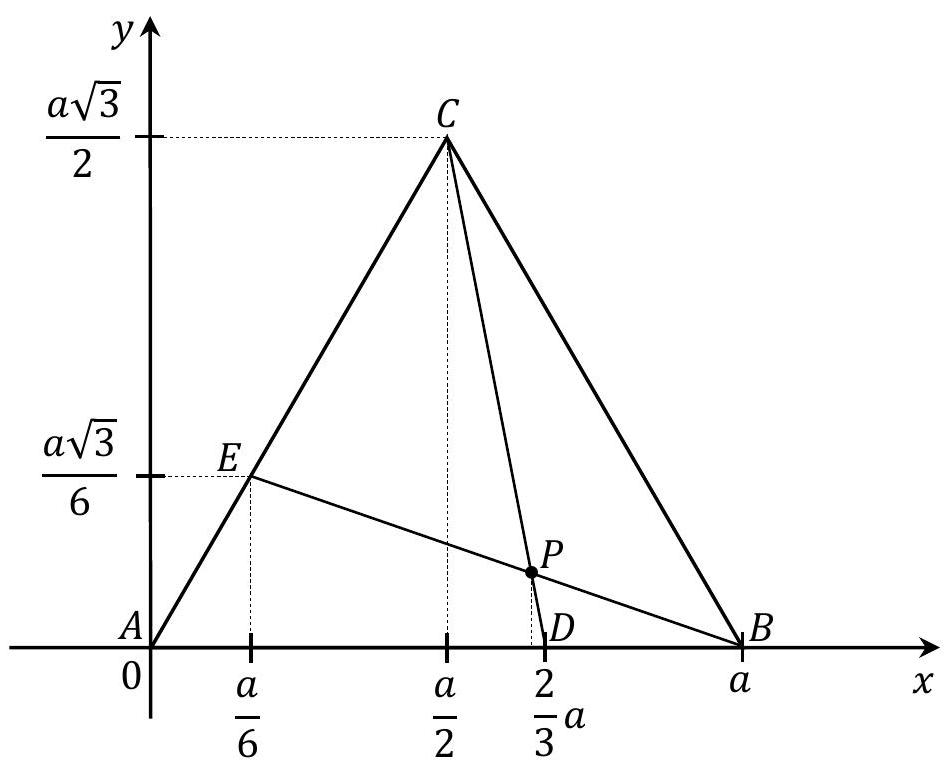
\includegraphics[max width=\textwidth, center]{2025_02_07_36131546116d12814c9cg-19}

Wtedy $C=\left(\frac{a}{2}, \frac{a \sqrt{3}}{2}\right), D=\left(\frac{2}{3} a, 0\right), E=\left(\frac{1}{3} \cdot \frac{a}{2}, \frac{1}{3} \cdot \frac{a \sqrt{3}}{2}\right)=\left(\frac{a}{6}, \frac{a \sqrt{3}}{6}\right)$.\\
Współczynniki kierunkowe prostych $C D$ i $B E$ są równe\\
$a_{C D}=\frac{\frac{a \sqrt{3}}{2}-0}{\frac{a}{2}-\frac{2}{3} a}=-3 \sqrt{3}$ oraz $a_{B E}=\frac{\frac{a \sqrt{3}}{6}-0}{\frac{a}{6}-a}=-\frac{\sqrt{3}}{5}$.\\
Zatem prosta $C D$ ma równanie $y=-3 \sqrt{3}\left(x-\frac{2}{3} a\right)$, natomiast prosta $B E$ ma równanie $y=-\frac{\sqrt{3}}{5}(x-a)$.\\
Obliczamy współrzędne punktu $P$, rozwiązując układ równań $\left\{\begin{array}{l}y=-3 \sqrt{3}\left(x-\frac{2}{3} a\right) \\ y=-\frac{\sqrt{3}}{5}(x-a)\end{array}\right.$. Stąd otrzymujemy $x=\frac{9}{14} a$ oraz $y=-\frac{\sqrt{3}}{5}\left(\frac{9}{14} a-a\right)=\frac{\sqrt{3}}{14} a$, więc $P=\left(\frac{9}{14} a, \frac{\sqrt{3}}{14} a\right)$. Zatem

$$
\frac{P_{D B P}}{P_{A B C}}=\frac{\frac{1}{2} \cdot|D B| \cdot \frac{\sqrt{3}}{14} a}{\frac{a^{2} \sqrt{3}}{4}}=\frac{\frac{1}{2} \cdot \frac{1}{3} a \cdot \frac{\sqrt{3}}{14} a}{\frac{a^{2} \sqrt{3}}{4}}=\frac{1}{21}
$$

czyli $P_{D B P}=\frac{1}{21} P_{A B C}$.\\
To należało wykazać.

\section*{Sposób 10.}
Trójkąt $A B C$ umieszczamy na sieci złożonej z przystających trójkątów równobocznych (jak na rysunku). Punkty $F, G, H, R, S$ to wybrane węzły sieci.\\
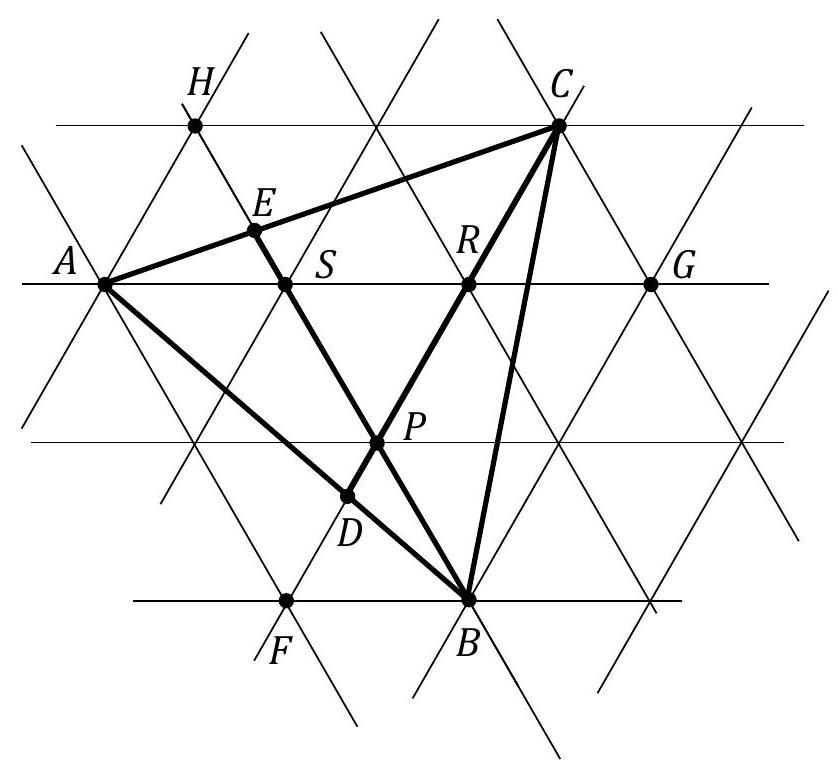
\includegraphics[max width=\textwidth, center]{2025_02_07_36131546116d12814c9cg-20}

Niech jednostką pola będzie pole jednego elementarnego trójkąta sieci.

Trójkąt $D B P$ jest podobny do trójkąta $D A F$ (cecha KKK), więc $\frac{|D P|}{|F D|}=\frac{|D B|}{|A D|}=\frac{1}{2}$. Stąd $|F D|=2|D P|$, więc $|D P|=\frac{1}{3}|P F|$. Trójkąty $D B P$ oraz $P F B$ mają wspólną wysokość opuszczoną z wierzchołka $B$, więc $\frac{P_{D B P}}{P_{P F B}}=\frac{|D P|}{|P F|}=\frac{1}{3}$, czyli $P_{D B P}=\frac{1}{3} P_{P F B}=\frac{1}{3}$.\\
Ponieważ

$$
P_{A B C}=P_{P R S}+P_{A B S}+P_{B C P}+P_{C A R}=P_{P R S}+\frac{1}{2} P_{A F B S}+\frac{1}{2} P_{B G C P}+\frac{1}{2} P_{A R C H}
$$

więc

$$
P_{A B C}=1+\frac{1}{2} \cdot 4+\frac{1}{2} \cdot 4+\frac{1}{2} \cdot 4=7
$$

Zatem $P_{D B P}=\frac{1}{21} P_{A B C}$. To należało wykazać.

\section*{Zadanie 9. (0-4)}
\begin{center}
\begin{tabular}{|l|l|}
\hline
\multicolumn{2}{|c|}{Wymagania egzaminacyjne 2021} \\
\hline
\multicolumn{1}{|c|}{Wymaganie ogólne} & \multicolumn{1}{c|}{Wymaganie szczegółowe} \\
\hline
III. Modelowanie matematyczne. & Zdający: \\
 & R10.2) oblicza prawdopodobieństwo \\
 & warunkowe. \\
\hline
\end{tabular}
\end{center}

\section*{Zasady oceniania}
\section*{Zdający otrzymuje}
\begin{itemize}
  \item zapisze liczbę wszystkich zdarzeń elementarnych: $|\Omega|=9000$
\end{itemize}

ALBO

\begin{itemize}
  \item zastosuje poprawną metodę zliczania elementów zbioru $B$, zawierającego wszystkie liczby naturalne czterocyfrowe podzielne przez 18 (np. poprzez wykorzystanie własności ciągu arytmetycznego, stosowanie cech podzielności liczb całkowitych)\\
ALBO
  \item zastosuje poprawną metodę zliczania elementów zbioru $A \cap B$ (np. poprzez wykorzystanie własności ciągu arytmetycznego, stosowanie cech podzielności liczb całkowitych)\\
ALBO
  \item zapisze, że jeżeli $A$ jest zdarzeniem polegającym na wylosowaniu liczby podzielnej przez 15, to iloczyn zdarzeńn $A \cap B$ oznacza wylosowanie liczby podzielnej przez 90
\end{itemize}

\section*{Zdający otrzymuje}
gdy:

\begin{itemize}
  \item obliczy liczbę zdarzeń elementarnych sprzyjających zdarzeniu $B:|B|=500$
\end{itemize}

ALBO

\begin{itemize}
  \item obliczy liczbę zdarzeń elementarnych sprzyjających zdarzeniu $A \cap B:|A \cap B|=100$\\
Zdający otrzymuje ..... 3 p.\\
gdy:
  \item obliczy liczbę zdarzeń elementarnych sprzyjających zdarzeniu $B$ oraz obliczy liczbę zdarzeń elementarnych sprzyjających zdarzeniu $A \cap B:|B|=500,|A \cap B|=100$
\end{itemize}

\section*{Zdający otrzymuje}
4 p. gdy zastosuje poprawną metodę i obliczy szukane prawdopodobieństwo warunkowe: $P(A \mid B)=\frac{18}{90}=\frac{1}{5}$.

\section*{Uwagi:}
\begin{enumerate}
  \item Jeśli zdający rozwiąże zadanie, rozpatrując wszystkie liczby naturalne spełniające warunek $1 \leq x \leq 9999$, to może otrzymać co najwyżej 2 punkty za całe rozwiązanie.
  \item Jeśli zdający, wyznaczając, ile jest liczb podzielnych przez 18 lub 15, rozważa, że są one mniejsze niż 9000, to może otrzymać co najwyżej 2 punkty za całe rozwiązanie.
  \item Ignorujemy zapis $P(A \mid B)=\frac{|A \cup B|}{|B|}$, jeżeli z rozwiązania zdającego jednoznacznie wynika, że zliczał wszystkie zdarzenia elementarne sprzyjające iloczynowi tych zdarzeń.
  \item Jeżeli w sposobie zliczania elementów zbioru $|B|$ (lub $|A \cap B|$ ) opartym na kolejnych wyrazach ciągu arytmetycznego zdający poprawnie ustala pierwszy i ostatni wyraz ciągu oraz różnicę tego ciągu, to przyjmujemy ten sposób zliczania jest poprawny. Jeżeli natomiast błędnie ustali pierwszy lub ostatni wyraz ciągu, lub różnicę tego ciągu, to sposób uznajemy za niepoprawny. Jeżeli zdający podzieli zbiór wszystkich liczb całkowitych czterocyfrowych na rozłączne niepuste podzbiory i zlicza liczby podzielne przez 18 (lub 90) w każdym z tych podzbiorów, to ten sposób uznajemy za poprawny tylko wtedy, gdy popełni błąd w zliczaniu co najwyżej w jednym z tych podzbiorów.
\end{enumerate}

\section*{Przykładowe pełne rozwiązanie}
Niech $A$ oznacza zdarzenie, że wylosowana liczba jest podzielna przez 15.\\
Niech $B$ oznacza zdarzenie, że wylosowana liczba jest podzielna przez 18.\\
W zadaniu mamy obliczyć prawdopodobieństwo $P(A \mid B)=\frac{P(A \cap B)}{P(B)}$.\\
Zbiór liczb naturalnych czterocyfrowych zawiera 9000 elementów, zatem $|\Omega|=9000$.\\
Do zbioru $B$ należą liczby: 1008, 1026, 1044, ..., $1008+(n-1) \cdot 18 \quad$ (gdzie $1008+(n-1) \cdot 18 \leq 9999$, a liczba naturalna $n$ jest liczbą elementów zbioru $B)$.\\
Ponieważ

$$
n \leq \frac{9999-1008}{18}+1=500,5
$$

więc $n=500$.\\
Zatem

$$
P(B)=\frac{500}{9000}=\frac{5}{90}=\frac{1}{18} .
$$

Zdarzenie $A \cap B$ zachodzi tylko wtedy, gdy wylosowana liczba jest jednocześnie podzielna przez 15 i przez 18, czyli przez 90.

Do zbioru $A \cap B$ należą zatem liczby: 1080, 1170, 1260, ..., $1080+(m-1) \cdot 90$ (gdzie $1080+(m-1) \cdot 90 \leq 9999$, a liczba naturalna $m$ jest liczbą elementów zbioru $A \cap B)$.\\
Ponieważ

$$
m \leq \frac{9999-1080}{90}+1=100,1
$$

więc $m=100$.\\
Zatem

$$
P(A \cap B)=\frac{100}{9000}=\frac{1}{90} .
$$

Z definicji prawdopodobieństwa warunkowego otrzymujemy

$$
P(A \mid B)=\frac{P(A \cap B)}{P(B)}=\frac{\frac{1}{90}}{\frac{1}{18}}=\frac{18}{90}=\frac{1}{5} .
$$

\section*{Zadanie 10. (0-4)}
\begin{center}
\begin{tabular}{|l|l|}
\hline
\multicolumn{2}{|c|}{Wymagania egzaminacyjne 2021} \\
\hline
\multicolumn{1}{|c|}{Wymaganie ogólne} & \multicolumn{1}{|c|}{Wymagania szczegółowe} \\
\hline
IV. Użycie i tworzenie strategii. & Zdający: \\
 & P8.1) wyznacza równanie prostej \\
 & przechodzącej przez dwa dane punkty \\
 & (w postaci kierunkowej lub ogólnej); \\
 & R8.1) oblicza odległość punktu od prostej. \\
\hline
\end{tabular}
\end{center}

\section*{Zasady oceniania}
\section*{Zdający otrzymuje}
1 p.\\
gdy:

\begin{itemize}
  \item wyznaczy równanie prostej $A B, \mathrm{np} .: y=-7 x+50$
\end{itemize}

ALBO

\begin{itemize}
  \item obliczy długość odcinka $A B$ oraz pole trójkąta $A O B:|A B|=15 \sqrt{2}, P_{\triangle A O B}=75$
\end{itemize}

ALBO

\begin{itemize}
  \item wyznaczy równanie prostej prostopadłej do $A B$ : $y=\frac{1}{7} x$
\end{itemize}

Zdający otrzymuje\\
2 p. gdy:

\begin{itemize}
  \item zapisze układ równań złożony z równań dwóch prostych: $\left\{\begin{array}{l}y=\frac{1}{7} x \\ y=-7 x+50\end{array}\right.$
\end{itemize}

ALBO

\begin{itemize}
  \item obliczy promień okręgu, korzystając ze wzoru na odległość punktu od prostej lub obliczając wysokość trójkąta $A O B: r=5 \sqrt{2}$\\
ALBO
  \item zapisze, że punkt styczności prostej $A B$ do okręgu ma współrzędne $P=\left(x_{0}, f\left(x_{0}\right)\right)$ i $f^{\prime}\left(x_{0}\right)=-7$, gdzie $f(x)=\sqrt{50-x^{2}}$ i $50-x^{2}>0$\\
ALBO
  \item zapisze odległość $g$ (lub kwadrat odległości) punktu $(0,0)$ od dowolnego punktu prostej $A B$ w zależności od jednej zmiennej, np. $g(x)=\sqrt{x^{2}+(-7 x+50)^{2}}$\\
ALBO
  \item wyznaczy równanie prostej $A B$ oraz poda współrzędne wektora prostopadłego do prostej $A B$
\end{itemize}

\section*{Zdający otrzymuje}
3 p. gdy zapisze równanie z jedną niewiadomą, prowadzące do obliczenia współrzędnych punktu styczności, np.: $\frac{1}{7} x=-7 x+50$ lub $x^{2}+\left(\frac{1}{7} x\right)^{2}=50$, lub $x^{2}+(-7 x+50)^{2}=50$, lub $\frac{-2 x}{2 \sqrt{50-x^{2}}}=-7$, lub $\sqrt{\left(x^{2}+(-7 x+50)^{2}\right)}=\frac{|7 \cdot 0+0-50|}{\sqrt{7^{2}+1^{2}}}$

\section*{Zdający otrzymuje}
4 p.\\
gdy zastosuje poprawną metodę i obliczy promień okręgu oraz współrzędne punktu styczności prostej $A B$ do okręgu: $r=5 \sqrt{2}, P=(7,1)$.

\section*{Uwagi:}
\begin{enumerate}
  \item Jeżeli zdający realizuje strategię rozwiązania i jedynym błędem zdającego, który jednak nie ułatwia zagadnienia na żadnym etapie rozwiązania, jest błąd polegający na:\\
a) zastosowaniu nieistniejącego wzoru $\sqrt{a^{2} \pm b^{2}}=a \pm b$ lub $(a \pm b)^{2}=a^{2} \pm b^{2}$\\
b) niepoprawnym użyciu współrzędnych punktów $A$ i $B$ przy wyznaczaniu równania prostej $A B$\\
c) niepoprawnym zastosowaniu wzoru na odległość punktu od prostej lub na odległość dwóch punktów, lub wzoru na pole trójkąta, lub równania okręgu\\
d) niepoprawnym wyznaczeniu współczynnika kierunkowego prostej prostopadłej do danej prostej\\
e) wyznaczeniu jednej $z$ niewiadomych $z$ równania $x^{2}+y^{2}=50$ bez koniecznych założeń to zdający otrzymuje co najwyżej 2 punkty za całe rozwiązanie.
  \item Jeżeli zdający wyznaczy równanie prostej $A B$ i obliczy promień okręgu stycznego do prostej $A B$, a następnie poda (bez obliczeń) współrzędne punktu styczności, to otrzymuje: - 3 punkty za całe rozwiązanie, jeśli nie sprawdzi rachunkiem, że punkt $P=(7,1)$ należy do prostej $A B$ oraz do prostej prostopadłej (lub do prostej $A B$ i okręgu)
\end{enumerate}

\begin{itemize}
  \item 4 punkty za całe rozwiązanie, jeśli sprawdzi, wykonując stosowne obliczenia, że punkt $P=(7,1)$ należy do prostej $A B$ oraz do prostej prostopadłej (lub do prostej $A B$ i okręgu).
\end{itemize}

\begin{enumerate}
  \setcounter{enumi}{2}
  \item Jeżeli zdający odczyta z rysunku współrzędne punktu styczności $P=(7,1)$ (bez obliczeń) i obliczy długość promienia, to otrzymuje 1 punkt za całe rozwiązanie. Jeżeli zdający nie sporządzi rysunku i poda bez stosownych obliczeń współrzędne punktu styczności $P=(7,1)$ i obliczy długość promienia, to otrzymuje $\mathbf{0}$ punktów za całe rozwiązanie.
\end{enumerate}

\section*{Przykładowe pełne rozwiązania}
\section*{Sposób 1.}
Wyznaczamy równanie prostej $A B$.\\
Niech $y=a x+b$ będzie równaniem kierunkowym prostej $A B$.\\
Punkty $A$ i $B$ leżą na tej prostej, więc:

$$
-6=8 a+b \quad \text { i } \quad 15=5 a+b
$$

Stąd $a=-7$ i $b=50$.\\
Prosta $A B$ ma równanie:

\begin{itemize}
  \item w postaci kierunkowej: $y=-7 x+50$;
  \item w postaci ogólnej: $7 x+y-50=0$.
\end{itemize}

Obliczamy odległość punktu $O$ od prostej $A B$ :

$$
d(O, A B)=\frac{|7 \cdot 0+0-50|}{\sqrt{7^{2}+1^{2}}}=\frac{50}{\sqrt{50}}=\sqrt{50}=5 \sqrt{2}
$$

Obliczona odległość jest długością promienia okręgu: $d(O, A B)=r=5 \sqrt{2}$.\\
Przez $P$ oznaczmy punkt styczności prostej $A B$ do okręgu.\\
Prosta $O P$ przechodzi przez punkt $O=(0,0)$ i jest prostopadła do prostej $A B$, więc ma równanie: $y=\frac{1}{7} x$.

Obliczamy współrzędne punktu $P$ :

$$
\left\{\begin{array}{l}
y=\frac{1}{7} x \\
y=-7 x+50
\end{array}\right.
$$

Rozwiązaniem tego układu jest para liczb $x=7$ i $y=1$, więc $P=(7,1)$.

\section*{Sposób 2. Przez układ z okregiem (1)}
Wyznaczamy równanie prostej $A B$ jak w sposobie 1.\\
Prosta $A B$ ma równanie:

\begin{itemize}
  \item w postaci kierunkowej: $y=-7 x+50$;
  \item w postaci ogólnej: $7 x+y-50=0$.
\end{itemize}

Obliczamy odległość punktu $O$ od prostej $A B$ :

$$
d(O, A B)=\frac{|7 \cdot 0+0-50|}{\sqrt{7^{2}+1^{2}}}=\frac{50}{\sqrt{50}}=\sqrt{50}=5 \sqrt{2}
$$

Obliczona odległość jest długością promienia okręgu: $d(O, A B)=r=5 \sqrt{2}$.\\
Równanie okręgu o środku w punkcie $O=(0,0)$ i promieniu $r=5 \sqrt{2}$ ma postać $x^{2}+y^{2}=50$. Przez $P$ oznaczmy punkt styczności prostej $A B$ do okręgu $x^{2}+y^{2}=50$.\\
Obliczamy wspórzędne punktu $P$ :

$$
\left\{\begin{array}{l}
y=-7 x+50 \\
x^{2}+y^{2}=50
\end{array}\right.
$$

Rozwiązaniem tego układu jest para liczb $x=7$ i $y=1$, więc $P=(7,1)$.

\section*{Sposób 3. Przez układ z okregiem (2)}
Wyznaczamy równanie prostej $A B$ jak w sposobie 1.\\
Prosta $A B$ ma równanie:

\begin{itemize}
  \item w postaci kierunkowej: $y=-7 x+50$;
  \item w postaci ogólnej: $7 x+y-50=0$.
\end{itemize}

Obliczamy odległość punktu $O$ od prostej $A B$ :

$$
d(O, A B)=\frac{|7 \cdot 0+0-50|}{\sqrt{7^{2}+1^{2}}}=\frac{50}{\sqrt{50}}=\sqrt{50}=5 \sqrt{2}
$$

Obliczona odległość jest długością promienia okręgu: $d(O, A B)=r=5 \sqrt{2}$.\\
Równanie okręgu o środku w punkcie $O=(0,0)$ i promieniu $r=5 \sqrt{2}$ ma postać $x^{2}+y^{2}=50$. Przez $P$ oznaczmy punkt styczności prostej $A B$ do okręgu $x^{2}+y^{2}=50$.\\
Prosta $O P$ przechodzi przez punkt $O=(0,0)$ i jest prostopadła do prostej $A B$, więc ma równanie: $y=\frac{1}{7} x$.\\
Obliczamy współrzędne punktu $P$ :

$$
\left\{\begin{array}{l}
y=\frac{1}{7} x \\
x^{2}+y^{2}=50
\end{array}\right.
$$

Rozwiązaniami tego układu są pary liczb: $\left\{\begin{array}{l}x=7 \\ y=1\end{array}\right.$ oraz $\left\{\begin{array}{l}x=-7 \\ y=-1\end{array}\right.$. Ponieważ punkt o współrzędnych $(-7,-1)$ nie należy do prostej o równaniu $y=-7 x+50$, więc $P=(7,1)$.

\section*{Sposób 4.}
Wyznaczamy równanie prostej $A B: y=-7 x+50$ (np. jak w sposobie 1.).\\
Obliczamy długość odcinka $A B$ :

$$
|A B|=\sqrt{(8-5)^{2}+(-6-15)^{2}}=\sqrt{9+441}=\sqrt{450}=15 \sqrt{2}
$$

Obliczamy pole trójkąta $A B O$ :

$$
P=\frac{1}{2}|(5-8)(0+6)-(15+6)(0-8)|=\frac{1}{2}|-18+168|=\frac{1}{2} \cdot 150=75
$$

Promień okręgu jest wysokością tego trójkąta poprowadzoną na bok $A B$, więc

$$
r=\frac{2 \cdot P}{|A B|}=\frac{2 \cdot 75}{15 \sqrt{2}}=\frac{150}{15 \sqrt{2}}=\frac{10}{\sqrt{2}}=5 \sqrt{2}
$$

Przez $P$ oznaczmy punkt styczności prostej $A B$ do okręgu $x^{2}+y^{2}=50$.\\
Obliczamy wspórzędne punktu $P$ :

$$
\left\{\begin{array}{l}
y=-7 x+50 \\
x^{2}+y^{2}=50
\end{array}\right.
$$

Rozwiązaniem tego układu jest para liczb $x=7$ i $y=1$, więc $P=(7,1)$.

\section*{Sposób 5. Punkt styczności przez pochodna}
Wyznaczamy równanie prostej $A B$ jak w sposobie 1.\\
Prosta $A B$ ma równanie:

\begin{itemize}
  \item w postaci kierunkowej: $y=-7 x+50$;
  \item w postaci ogólnej: $7 x+y-50=0$.
\end{itemize}

Obliczamy odległość punktu $O$ od prostej $A B$ :

$$
d(O, A B)=\frac{|7 \cdot 0+0-50|}{\sqrt{7^{2}+1^{2}}}=\frac{50}{\sqrt{50}}=\sqrt{50}=5 \sqrt{2}
$$

Obliczona odległość jest długością promienia okręgu: $d(O, A B)=r=5 \sqrt{2}$.\\
Równanie okręgu o środku w punkcie $O=(0,0)$ i promieniu $r=5 \sqrt{2}$ ma postać $x^{2}+y^{2}=50$. Przez $P$ oznaczmy punkt styczności prostej $A B$ do okręgu $x^{2}+y^{2}=50$. Punkt $P$ leży w I ćwiartce układu wspórrzędnych (ponieważ prosta $A B$ przechodzi przez I, II i IV ćwiartkę układu wspórrzędnych), więc punkt $P$ należy do wykresu funkcji $f$ określonej wzorem $f(x)=\sqrt{50-x^{2}}$, gdzie $50-x^{2}>0$. Zatem $P=\left(x_{0}, f\left(x_{0}\right)\right)$, przy pewnym $x_{0}$ takim, że $50-x_{0}^{2}>0$ oraz $f^{\prime}\left(x_{0}\right)=-7$.\\
Obliczamy wspórzędne punktu $P$ :

$$
\begin{gathered}
f^{\prime}(x)=\frac{-2 x}{2 \sqrt{50-x^{2}}} \\
-7=\frac{-x}{\sqrt{50-x^{2}}} \quad \text { i } \quad 50-x^{2}>0
\end{gathered}
$$

Stąd otrzymujemy $x=7$. Zatem $P=(7, f(7))=(7,1)$.

\section*{Sposób 6.}
Wyznaczamy równanie prostej $A B$ jak w sposobie 1.\\
Przez $P$ oznaczmy punkt styczności prostej $A B$ do okręgu.\\
Wektor $\overrightarrow{O P}$ jest wektorem prostopadłym do prostej $A B$, więc jest postaci [7t, t], przy pewnym $t \neq 0$. Zatem punkt $P$ ma wspórzzędne $P=(7 t, t)$.\\
Punkt $P$ należy do prostej $A B$, więc $7 \cdot 7 t+t-50=0$. Stąd $t=1$ i $P=(7,1)$. Promień okręgu jest zatem równy $r=|O P|=\sqrt{7^{2}+1^{2}}=5 \sqrt{2}$.

\section*{Zadanie 11. (0-5)}
\begin{center}
\begin{tabular}{|l|l|}
\hline
\multicolumn{2}{|c|}{Wymagania egzaminacyjne 2021} \\
\hline
\multicolumn{1}{|c|}{Wymaganie ogólne} & \multicolumn{1}{c|}{Wymagania szczegółowe} \\
\hline
IV. Użycie i tworzenie strategii. & Zdający: \\
 & R3.1) stosuje wzory Viète'a; \\
 & R3.2) rozwiązuje równania i nierówności \\
 & liniowe i kwadratowe z parametrem; \\
 & R3.7) rozwiązuje proste nierówności \\
 & wymierne [...]. \\
\hline
\end{tabular}
\end{center}

\section*{Zasady oceniania}
Rozwiązanie składa się z trzech etapów.\\
Pierwszy etap polega na rozwiązaniu nierówności $\Delta>0: m \neq 1$.\\
Za poprawne rozwiązanie tego etapu zdający otrzymuje 1 punkt.

\section*{Uwaga do pierwszego etapu:}
Jeżeli zdający rozwiązuje nierówność $\Delta \geq 0$, to za pierwszy etap otrzymuje $\mathbf{0}$ punktów.\\
Drugi etap polega na rozwiązaniu nierówności $x_{1}+x_{2} \leq \frac{1}{x_{1}}+\frac{1}{x_{2}}$.\\
Za poprawne rozwiązanie drugiego etapu zdający otrzymuje 3 punkty.\\
Podział punktów za drugi etap rozwiązania:

1 punkt zdający otrzymuje, gdy:

\begin{itemize}
  \item przekształci nierówność $x_{1}+x_{2} \leq \frac{1}{x_{1}}+\frac{1}{x_{2}}$ do postaci $x_{1}+x_{2} \leq \frac{x_{1}+x_{2}}{x_{1} \cdot x_{2}}$ lub
\end{itemize}

$$
\left(x_{1}+x_{2}\right) \cdot\left(x_{1} x_{2}\right)^{2} \leq\left(x_{1}+x_{2}\right) x_{1} x_{2}
$$

ALBO

\begin{itemize}
  \item wyznaczy pierwiastki trójmianu $4 x^{2}-2(m+1) x+m: x_{1}=\frac{1}{2}, x_{2}=\frac{m}{2}$.
\end{itemize}

2 punkty zdający otrzymuje, gdy zapisze nierówność z jedną niewiadomą $m$ :

$$
\frac{2(m+1)}{4} \leq \frac{\frac{2(m+1)}{4}}{\frac{m}{4}} \text { lub } \frac{1}{2}+\frac{m}{2} \leq 2+\frac{2}{m} \text { lub } \frac{2(m+1)}{4} \cdot\left(\frac{m}{4}\right)^{2} \leq \frac{2(m+1)}{4} \cdot \frac{m}{4}
$$

3 punkty zdający otrzymuje, gdy rozwiąże nierówność $\frac{2(m+1)}{4} \leq \frac{\frac{2(m+1)}{4}}{\frac{m}{4}}$ :\\
$m \in(-\infty,-1\rangle \cup(0,4\rangle$.

\section*{Uwagi do drugiego etapu:}
\begin{enumerate}
  \item Jeżeli zdający, rozwiązując nierównośćć $\frac{2(m+1)}{4} \leq \frac{\frac{2(m+1)}{4}}{\frac{m}{4}}$, nie uwzględni warunku $m \neq 0$, to za drugi etap może otrzymać co najwyżej 2 punkty.
  \item Jeżeli zdający:
\end{enumerate}

\begin{itemize}
  \item mnoży nierówność $x_{1}+x_{2} \leq \frac{1}{x_{1}}+\frac{1}{x_{2}}$ stronami przez iloczyn $x_{1} \cdot x_{2}$ bez rozpatrzenia znaku tego iloczynu\\
ALBO
  \item dzieli nierówność $x_{1}+x_{2} \leq \frac{x_{1}+x_{2}}{x_{1} \cdot x_{2}}$ stronami przez sumę $x_{1}+x_{2}$ bez rozpatrzenia znaku tej sumy\\
to za drugi etap może otrzymać co najwyżej 1 punkt.\\
Trzeci etap polega na wyznaczeniu szukanych wartości parametru $m$ :\\
$m \in(-\infty,-1\rangle \cup(0,1) \cup(1,4\rangle$.\\
Za poprawne rozwiązanie tego etapu zdający otrzymuje 1 punkt.
\end{itemize}

\section*{Uwagi do trzeciego etapu:}
\begin{enumerate}
  \item Jeżeli zdający popełni błędy rachunkowe w etapach I i II (nie otrzymując pustego zbioru rozwiązań ani zbioru $\mathbb{R}$ wszystkich liczb rzeczywistych), lecz konsekwentnie wyznaczy iloczyn w etapie III, to za III etap otrzymuje 1 punkt.
  \item Zdający może otrzymać 1 punkt za III etap, jeżeli jedynymi błędami jakie popełni w I i II etapie są błędy rachunkowe.
\end{enumerate}

\section*{Przykładowe pełne rozwiązanie}
\section*{I etap}
Trójmian $4 x^{2}-2(m+1) x+m$ ma dwa różne pierwiastki rzeczywiste wtedy i tylko wtedy, gdy jego wyróżnik jest dodatni, czyli

$$
\Delta=[-2(m+1)]^{2}-4 \cdot 4 \cdot m>0
$$

i równoważnie dalej

$$
\begin{gathered}
4 m^{2}-8 m+4>0 \\
4(m-1)^{2}>0 \\
m \neq 1
\end{gathered}
$$

\section*{II etap}
Warunek $x_{1}+x_{2} \leq \frac{1}{x_{1}}+\frac{1}{x_{2}}$ ma sens liczbowy tylko wtedy, gdy żaden $z$ pierwiastków trójmianu $4 x^{2}-2(m+1) x+m$ nie jest równy 0 , czyli gdy $x_{1} x_{2} \neq 0$. Ze wzoru Viète'a otrzymujemy $\frac{m}{4} \neq 0$, czyli $m \neq 0$.\\
Nierówność $x_{1}+x_{2} \leq \frac{1}{x_{1}}+\frac{1}{x_{2}}$ zapisujemy w postaci równoważnej $x_{1}+x_{2} \leq \frac{x_{1}+x_{2}}{x_{1} \cdot x_{2}}$ i po zastosowaniu wzorów Viète'a otrzymujemy

$$
\frac{2(m+1)}{4} \leq \frac{\frac{2(m+1)}{4}}{\frac{m}{4}}
$$

i równoważnie dalej

$$
\begin{gathered}
\frac{(m+1)}{2} \leq \frac{2(m+1)}{m} \\
\frac{2(m+1)}{m}-\frac{m+1}{2} \geq 0 \\
\frac{4(m+1)-m(m+1)}{2 m} \geq 0 \\
2 m(m+1)(4-m) \geq 0 \text { i } m \neq 0
\end{gathered}
$$

Stąd $m \in(-\infty,-1) \cup(0,4\rangle$.

\section*{III etap}
Wyznaczamy część wspólną zbiorów rozwiązań nierówności otrzymanych w I i II etapie rozwiązania: $m \in(-\infty,-1\rangle \cup(0,1) \cup(1,4\rangle$.

\section*{Uwaga:}
Zamiast korzystać ze wzorów Viète'a, możemy wzór trójmianu $4 x^{2}-2(m+1) x+m$ zapisać w postaci równoważnej:

$$
4 x^{2}-2 m x-2 x+m=2 x(2 x-m)-(2 x-m)=(2 x-1)(2 x-m)
$$

Stąd wynika, że pierwiastkami tego trójmianu są liczby $x_{1}=\frac{1}{2}$ oraz $x_{2}=\frac{m}{2}$ dla każdej wartości parametru $m$. Pierwiastki są różne wtedy i tylko wtedy, gdy $m \neq 1$.\\
Pierwiastki te można też wyznaczyć, korzystając ze wzorów na pierwiastki trójmianu kwadratowego. Ponieważ wyróżnik $\Delta$ trójmianu $4 x^{2}-2(m+1) x+m$ jest kwadratem wyrażenia $2(m-1)$, więc

$$
\begin{aligned}
& x_{1}=\frac{2(m+1)-2(m-1)}{2 \cdot 4}=\frac{1}{2} \\
& x_{2}=\frac{2(m+1)+2(m-1)}{2 \cdot 4}=\frac{m}{2}
\end{aligned}
$$

Wtedy nierówność $x_{1}+x_{2} \leq \frac{1}{x_{1}}+\frac{1}{x_{2}}$ przyjmie postać $\frac{1}{2}+\frac{m}{2} \leq 2+\frac{2}{m}$\\
Nierówność ta ma sens liczbowy tylko dla $m \neq 0$.\\
Przekształcając nierówność $\frac{1}{2}+\frac{m}{2} \leq 2+\frac{2}{m}$, otrzymujemy kolejno

$$
\begin{gathered}
\frac{m}{2}-\frac{2}{m}-\frac{3}{2} \leq 0 \\
\frac{m^{2}-3 m-4}{2 m} \leq 0
\end{gathered}
$$

$$
\begin{gathered}
\frac{(m+1)(m-4)}{2 m} \leq 0 \\
2 m(m+1)(m-4) \leq 0 \quad \text { i } \quad m \neq 0
\end{gathered}
$$

Stąd $m \in(-\infty,-1) \cup(0,4\rangle$.\\
Uwzględniając uzyskany wcześniej warunek $m \neq 1$, otrzymujemy ostatecznie $m \in(-\infty,-1\rangle \cup(0,1) \cup(1,4\rangle$.

\section*{Zadanie 12. (0-5)}
\begin{center}
\begin{tabular}{|l|l|}
\hline
\multicolumn{2}{|c|}{Wymagania egzaminacyjne 2021} \\
\hline
\multicolumn{1}{|c|}{Wymaganie ogólne} & \multicolumn{1}{|c|}{Wymaganie szczegółowe} \\
\hline
IV. Użycie i tworzenie strategii. & Zdający: \\
 & R6.6) rozwiązuje równania \\
 & trygonometryczne [...]. \\
\hline
\end{tabular}
\end{center}

\section*{Zasady oceniania}
Zdający otrzymuje\\
1 p.\\
gdy:

\begin{itemize}
  \item zapisze alternatywę równań $\cos x-\sin x=0$ lub $\cos x+\sin x=\frac{\sqrt{2}}{2}$
\end{itemize}

ALBO

\begin{itemize}
  \item zastosuje wzór na cosinus podwojonego argumentu i zapisze równanie $\cos 2 x=\frac{\sqrt{2}}{2}(\cos x-\sin x)$ w postaci
\end{itemize}

$$
(\cos x-\sin x)(\cos x+\sin x)=\frac{\sqrt{2}}{2}(\cos x-\sin x)
$$

ALBO

\begin{itemize}
  \item zapisze równanie $\cos 2 x=\frac{\sqrt{2}}{2}(\cos x-\sin x)$ w postaci $\cos 2 x=\cos x \cdot \cos \frac{\pi}{4}-\sin x \cdot \sin \frac{\pi}{4}$ lub $\cos 2 x=\cos x \cdot \sin \frac{\pi}{4}-\sin x \cdot \cos \frac{\pi}{4}$
\end{itemize}

Zdający otrzymuje 2 p. gdy:

\begin{itemize}
  \item zapisze alternatywę równań $\cos x-\sin x=0$ lub $\cos x+\sin x=\frac{\sqrt{2}}{2}$ i spełni jeden z poniższych warunków:
\end{itemize}

\begin{enumerate}
  \item rozwiąże równanie $\cos x-\sin x=0: \quad x=\frac{\pi}{4}+k \pi$, gdzie $k$ jest liczbą całkowitą, lub $x=\frac{\pi}{4}$,
  \item przekształci równanie $\cos x+\sin x=\frac{\sqrt{2}}{2}$ do postaci $\cos \left(\frac{\pi}{4}-x\right)=\frac{1}{2}$,
  \item skorzysta $z_{\text {,jedynki trygonometrycznej", zapisze układ równań }}\left\{\begin{array}{c}\cos x+\sin x=\frac{\sqrt{2}}{2} \\ \sin ^{2} x+\cos ^{2} x=1\end{array}\right.$ i przekształci go do równania, w którym występuje jedna funkcja trygonometryczna zmiennej $x$ :
\end{enumerate}

$$
\begin{aligned}
& \left(\frac{\sqrt{2}}{2}-\cos x\right)^{2}+\cos ^{2} x=1 \text { lub } \sin ^{2} x+\left(\frac{\sqrt{2}}{2}-\sin x\right)^{2}=1 \\
& \text { lub } 2 \cos ^{2} x-\sqrt{2} \cos x-\frac{1}{2}=0 \quad \text { lub } 2 \sin ^{2} x-\sqrt{2} \sin x-\frac{1}{2}=0
\end{aligned}
$$

ALBO

\begin{itemize}
  \item przekształci równanie $\cos 2 x=\frac{\sqrt{2}}{2}(\cos x-\sin x)$ do postaci $\cos 2 x=\cos \left(x+\frac{\pi}{4}\right)$
\end{itemize}

Zdający otrzymuje $\qquad$ 3 p. gdy:

\begin{itemize}
  \item rozwiąże równanie $\cos x-\sin x=0: x=\frac{\pi}{4}+k \pi$, gdzie $k$ jest liczbą całkowitą, lub $x=\frac{\pi}{4}$ oraz spełni jeden $z$ poniższych warunków:
\end{itemize}

\begin{enumerate}
  \item przekształci równanie $\cos x+\sin x=\frac{\sqrt{2}}{2}$ do postaci $\cos \left(\frac{\pi}{4}-x\right)=\frac{1}{2}$
  \item skorzysta $z$,jedynki trygonometrycznej", zapisze układ równań $\left\{\begin{array}{c}\cos x+\sin x=\frac{\sqrt{2}}{2} \\ \sin ^{2} x+\cos ^{2} x=1\end{array}\right.$\\
i przekształci go do równania, w którym występuje jedna funkcja trygonometryczna zmiennej $x$ :
\end{enumerate}

$$
\begin{aligned}
& \left(\frac{\sqrt{2}}{2}-\cos x\right)^{2}+\cos ^{2} x=1 \text { lub } \sin ^{2} x+\left(\frac{\sqrt{2}}{2}-\sin x\right)^{2}=1 \\
& \text { lub } 2 \cos ^{2} x-\sqrt{2} \cos x-\frac{1}{2}=0 \quad \text { lub } 2 \sin ^{2} x-\sqrt{2} \sin x-\frac{1}{2}=0
\end{aligned}
$$

ALBO

\begin{itemize}
  \item zapisze alternatywę równań $\cos x-\sin x=0$ lub $\cos x+\sin x=\frac{\sqrt{2}}{2}$ oraz zapisze poprawnie jedną serię rozwiązań równania $\cos x+\sin x=\frac{\sqrt{2}}{2}$ : $\frac{\pi}{4}-x=\frac{\pi}{3}+2 k \pi$ lub $\frac{\pi}{4}-x=-\frac{\pi}{3}+2 k \pi$, gdzie $k$ jest liczbą całkowitą ALBO
  \item zapisze poprawnie jedną serię rozwiązań równania $\cos 2 x=\cos \left(x+\frac{\pi}{4}\right)$ : $2 x=x+\frac{\pi}{4}+2 k \pi$ lub $2 x=-\left(x+\frac{\pi}{4}\right)+2 k \pi$, gdzie $k$ jest liczbą całkowitą (bez wyznaczenia rozwiązań z danego przedziału), albo zapisze poprawnie jedno rozwiązanie w przedziale $\langle 0, \pi\rangle$ : $\frac{\pi}{4}$ lub $\frac{7 \pi}{12}$.\\
ALBO
  \item zastosuje wzór na różnicę cosinusów i przekształci równanie $\cos 2 x=\cos \left(x+\frac{\pi}{4}\right)$ do postaci:
\end{itemize}

$$
-2 \sin \left(\frac{2 x+x+\frac{\pi}{4}}{2}\right) \cdot \sin \left(\frac{2 x-x-\frac{\pi}{4}}{2}\right)=0
$$

\section*{Zdający otrzymuje}
 4 p. gdy:\begin{itemize}
  \item rozwiąże równanie $\cos x-\sin x=0 \quad$ w przedziale $\langle 0, \pi\rangle: \frac{\pi}{4} \quad$ i spełni jeden z poniższych warunków:
\end{itemize}

\begin{enumerate}
  \item rozwiąże równanie $\cos \left(\frac{\pi}{4}-x\right)=\frac{1}{2}$ i poda dwie serie rozwiązań:\\
$\frac{\pi}{4}-x=\frac{\pi}{3}+2 k \pi$ oraz $\frac{\pi}{4}-x=-\frac{\pi}{3}+2 k \pi$, gdzie $k$ jest liczbą całkowitą (bez wyznaczenia rozwiązań $z$ danego przedziału)
  \item przekształci równanie $2 \sin ^{2} x-\sqrt{2} \sin x-\frac{1}{2}=0$ do alternatywy:\\
$\sin x=\frac{\sqrt{2}+\sqrt{6}}{4}$ lub $\sin x=\frac{\sqrt{2}-\sqrt{6}}{4}$\\
ALBO\\
przekształci równanie $2 \cos ^{2} x-\sqrt{2} \cos x-\frac{1}{2}=0$ do alternatywy:\\
$\cos x=\frac{\sqrt{2}+\sqrt{6}}{4}$ lub $\cos x=\frac{\sqrt{2}-\sqrt{6}}{4}$\\
ALBO
\end{enumerate}

\begin{itemize}
  \item zapisze poprawnie dwie serie rozwiązań równania $\cos 2 x=\cos \left(x+\frac{\pi}{4}\right)$ : $2 x=x+\frac{\pi}{4}+2 k \pi$ oraz $2 x=-\left(x+\frac{\pi}{4}\right)+2 k \pi$, gdzie $k$ jest liczbą całkowitą (bez wyznaczenia rozwiązań $z$ danego przedziału)\\
ALBO
  \item rozwiąże równanie $\sin \left(\frac{3}{2} x+\frac{\pi}{8}\right)=0 \mathrm{w}$ przedziale $\langle 0, \pi\rangle: \frac{7 \pi}{12}$
\end{itemize}

ALBO

\begin{itemize}
  \item rozwiąże równanie $\sin \left(\frac{1}{2} x-\frac{\pi}{8}\right)=0$ w przedziale $\langle 0, \pi\rangle: \frac{\pi}{4}$
\end{itemize}

ALBO

\begin{itemize}
  \item zapisze poprawnie dwie serie rozwiązań równań $\sin \left(\frac{3}{2} x+\frac{\pi}{8}\right)=0$ i $\sin \left(\frac{1}{2} x-\frac{\pi}{8}\right)=0$ : $x=-\frac{\pi}{12}+\frac{2}{3} k \pi$ oraz $x=\frac{\pi}{4}+2 k \pi$, gdzie $k$ jest liczbą całkowita
\end{itemize}

\section*{Zdający otrzymuje}
 5 p.gdy zastosuje poprawną metodę rozwiązania równania $\cos 2 x=\frac{\sqrt{2}}{2}(\cos x-\sin x)$ i poda prawidłowe rozwiązania w przedziale $\langle 0, \pi\rangle: \frac{\pi}{4}, \frac{7 \pi}{12}$.

\section*{Uwagi:}
\begin{enumerate}
  \item Jeśli zdający zapisze równanie
\end{enumerate}

$$
(\cos x-\sin x)(\cos x+\sin x)=\frac{\sqrt{2}}{2}(\cos x-\sin x)
$$

i podzieli obie strony równania przez $\cos x-\sin x \quad$ (bez rozstrzygania sytuacji, gdy $\cos x=\sin x$ ), otrzyma równanie $\cos x+\sin x=\frac{\sqrt{2}}{2}$ i doprowadzi rozwiązanie do końca, to traktujemy to jako błąd merytoryczny, nie przekreślający całości rozwiązania i zdający może otrzymać co najwyżej 3 punkty za całe rozwiązanie.\\
2. Jeżeli jedynym błędem zdającego jest błąd przy przepisywaniu wzoru trygonometrycznego, np. zapisuje sinus sumy argumentów zamiast sinusa ich różnicy, i konsekwentnie doprowadzi rozwiązanie do końca, to zdający może otrzymać 3 punkty za całe rozwiązanie.\\
3. Jeżeli zdający, rozwiązując jedno $z$ otrzymanych równań, stosuje metodę analizy starożytnych, np. podnosi obie strony równania $\cos x+\sin x=\frac{\sqrt{2}}{2}$ do kwadratu i nie odrzuci rozwiązań obcych, to za całe rozwiązanie może otrzymać co najwyżej 3 punkty.

\section*{Przykładowe pełne rozwiązania}
\section*{Sposób 1.}
\section*{Ponieważ}
$$
\frac{\sqrt{2}}{2}(\cos x-\sin x)=\cos x \cdot \frac{\sqrt{2}}{2}-\sin x \cdot \frac{\sqrt{2}}{2}=\cos x \cdot \cos \frac{\pi}{4}-\sin x \cdot \sin \frac{\pi}{4}=\cos \left(x+\frac{\pi}{4}\right)
$$

więc równanie $\cos 2 x=\frac{\sqrt{2}}{2}(\cos x-\sin x)$ można zapisać $w$ postaci równoważnej

$$
\cos 2 x=\cos \left(x+\frac{\pi}{4}\right)
$$

Jego rozwiązaniami są liczby $x$ spełniające warunek

$$
2 x=x+\frac{\pi}{4}+2 k \pi \quad \text { lub } \quad 2 x=-\left(x+\frac{\pi}{4}\right)+2 k \pi
$$

gdzie $k$ jest liczbą całkowitą.\\
Stąd $x=\frac{\pi}{4}+2 k \pi$ lub $3 x=-\frac{\pi}{4}+2 k \pi$, czyli $x=\frac{\pi}{4}+2 k \pi$ lub $x=-\frac{\pi}{12}+\frac{2}{3} k \pi$.\\
Zatem rozwiązaniami równania $\cos 2 x=\frac{\sqrt{2}}{2}(\cos x-\sin x)$ w przedziale $\langle 0, \pi\rangle$ są liczby: $\frac{\pi}{4}$ oraz $\frac{7 \pi}{12}$.

\section*{Sposób 2.}
Po skorzystaniu ze wzoru na cosinus podwojonego argumentu otrzymujemy równanie

$$
(\cos x-\sin x)(\cos x+\sin x)=\frac{\sqrt{2}}{2}(\cos x-\sin x)
$$

Jest ono równoważne alternatywie dwóch równań:

$$
\cos x-\sin x=0 \quad \text { lub } \quad \cos x+\sin x=\frac{\sqrt{2}}{2}
$$

Równanie $\cos x-\sin x=0$ można rozwiązać graficznie albo algebraicznie, zapisując je z wykorzystaniem wzoru redukcyjnego np. w postaci $\cos x=\cos \left(\frac{\pi}{2}-x\right)$. Rozwiązaniami\\
ostatniego równania są liczby spetniające warunek $x=\frac{\pi}{2}-x+2 k \pi$ lub $x=-\left(\frac{\pi}{2}-x\right)+2 k \pi$, gdzie $k$ jest dowolną liczbą całkowitą. Stąd $x=\frac{\pi}{4}+k \pi$, gdzie $k$ jest dowolną liczbą całkowitą, więc rozwiązaniem równania $\cos x-\sin x=0 \mathrm{w}$ przedziale $\langle 0, \pi\rangle$ jest liczba $\frac{\pi}{4}$. Równanie $\cos x+\sin x=\frac{\sqrt{2}}{2}$ rozwiązujemy, stosując wzory redukcyjne oraz wzór na sumę sinusów. Otrzymujemy kolejno:

$$
\begin{gathered}
\sin \left(\frac{\pi}{2}-x\right)+\sin x=\frac{\sqrt{2}}{2} \\
2 \sin \left(\frac{\frac{\pi}{2}-x+x}{2}\right) \cdot \cos \left(\frac{\frac{\pi}{2}-x-x}{2}\right)=\frac{\sqrt{2}}{2} \\
2 \sin \left(\frac{\pi}{4}\right) \cdot \cos \left(\frac{\pi}{4}-x\right)=\frac{\sqrt{2}}{2} \\
\cos \left(\frac{\pi}{4}-x\right)=\frac{1}{2}
\end{gathered}
$$

Rozwiązaniami otrzymanego równania są liczby spełniające warunek $\frac{\pi}{4}-x=\frac{\pi}{3}+2 k \pi$ lub $\frac{\pi}{4}-x=-\frac{\pi}{3}+2 k \pi$, gdzie $k$ jest dowolną liczbą całkowita. Stąd $x=-\frac{\pi}{12}+2 k \pi$ lub $x=\frac{7 \pi}{12}+2 k \pi$, gdzie $k$ jest dowolną liczbą całkowitą.\\
Zatem rozwiązaniem równania $\cos \left(\frac{\pi}{4}-x\right)=\frac{1}{2} \mathrm{w}$ przedziale $\langle 0, \pi\rangle$ jest liczba $\frac{7 \pi}{12}$.\\
Ostatecznie, rozwiązaniami równania $\cos 2 x=\frac{\sqrt{2}}{2}(\cos x-\sin x) \mathrm{w}$ przedziale $\langle 0, \pi\rangle$ są liczby $\frac{\pi}{4}$ oraz $\frac{7 \pi}{12}$.

Sposób 3. Po skorzystaniu ze wzoru na cosinus podwojonego argumentu otrzymujemy równanie

$$
(\cos x-\sin x)(\cos x+\sin x)=\frac{\sqrt{2}}{2}(\cos x-\sin x)
$$

Jest ono równoważne alternatywie dwóch równań:

$$
\cos x-\sin x=0 \quad \text { lub } \quad \cos x+\sin x=\frac{\sqrt{2}}{2}
$$

Równanie $\cos x-\sin x=0$ można rozwiązać graficznie albo algebraicznie, zapisując je z wykorzystaniem wzoru redukcyjnego np . w postaci $\cos x=\cos \left(\frac{\pi}{2}-x\right)$. Rozwiązaniami ostatniego równania są liczby spelniające warunek $x=\frac{\pi}{2}-x+2 k \pi$ lub $x=-\left(\frac{\pi}{2}-x\right)+2 k \pi$, gdzie $k$ jest dowolną liczbą całkowitą. Stąd $x=\frac{\pi}{4}+k \pi$, gdzie $k$ jest dowolną liczbą całkowitą, więc rozwiązaniem równania $\cos x-\sin x=0 \mathrm{w}$ przedziale $\langle 0, \pi\rangle$ jest liczba $\frac{\pi}{4}$. Równanie $\cos x+\sin x=\frac{\sqrt{2}}{2}$ rozwiązujemy, stosując wzór $\cos ^{2} x+\sin ^{2} x=1$.

Zapisujemy układ równań

$$
\left\{\begin{array}{l}
\cos x+\sin x=\frac{\sqrt{2}}{2} \\
\cos ^{2} x+\sin ^{2} x=1
\end{array}\right.
$$

Stąd otrzymujemy kolejno

$$
\begin{gathered}
\left(\frac{\sqrt{2}}{2}-\sin x\right)^{2}+\sin ^{2} x-1=0 \\
2 \sin ^{2} x-\sqrt{2} \sin x-\frac{1}{2}=0
\end{gathered}
$$

Podstawiamy $\sin x=t$ i wtedy $2 t^{2}-\sqrt{2} t-\frac{1}{2}=0$.\\
Rozwiązaniami tego równania są $t=\frac{\sqrt{2}+\sqrt{6}}{4}$ lub $t=\frac{\sqrt{2}-\sqrt{6}}{4}$.\\
Ponieważ

$$
\frac{\sqrt{2}+\sqrt{6}}{4}=\frac{\sqrt{2}}{2} \cdot \frac{1}{2}+\frac{\sqrt{2}}{2} \cdot \frac{\sqrt{3}}{2}=\sin 45^{\circ} \cdot \cos 60^{\circ}+\cos 45^{\circ} \cdot \sin 60^{\circ}=\sin 105^{\circ}
$$

i $\sin 105^{\circ}+\cos 105^{\circ}=\frac{\sqrt{2}}{2}$, więc $x=105^{\circ}=\frac{7 \pi}{12}$ jest rozwiązaniem równania $\cos x+\sin x=\frac{\sqrt{2}}{2} \mathrm{w}$ przedziale $\langle 0, \pi\rangle$.\\
Ponieważ $\frac{\sqrt{2}-\sqrt{6}}{4}<0$, więc równanie $\sin x=\frac{\sqrt{2}-\sqrt{6}}{4}$ nie ma rozwiązań $w$ przedziale $\langle 0, \pi\rangle$.\\
Ostatecznie, rozwiązaniami równania $\cos 2 x=\frac{\sqrt{2}}{2}(\cos x-\sin x)$ w przedziale $\langle 0, \pi\rangle$ są liczby $\frac{\pi}{4}$ oraz $\frac{7 \pi}{12}$.

\section*{Sposób 4.}
Przekształcamy równanie jak w sposobie 1. do postaci $\cos 2 x=\cos \left(x+\frac{\pi}{4}\right)$, skąd

$$
\cos 2 x-\cos \left(x+\frac{\pi}{4}\right)=0
$$

Stosujemy wzór na różnicę cosinusów i otrzymujemy:

$$
-2 \sin \left(\frac{2 x+x+\frac{\pi}{4}}{2}\right) \cdot \sin \left(\frac{2 x-x-\frac{\pi}{4}}{2}\right)=0
$$

Stąd

$$
\sin \left(\frac{3}{2} x+\frac{\pi}{8}\right)=0 \text { lub } \sin \left(\frac{1}{2} x-\frac{\pi}{8}\right)=0
$$

więc $\frac{3}{2} x+\frac{\pi}{8}=k \pi$ lub $\frac{1}{2} x-\frac{\pi}{8}=k \pi$, gdzie $k$ jest liczbą całkowitą, czyli $x=-\frac{\pi}{12}+\frac{2}{3} k \pi$ lub $x=\frac{\pi}{4}+2 k \pi$, gdzie $k$ jest liczbą całkowita.\\
Rozwiązaniami równania $\cos 2 x=\cos \left(x+\frac{\pi}{4}\right)$ w przedziale $\langle 0, \pi\rangle$ są liczby $\frac{7 \pi}{12}$ oraz $\frac{\pi}{4}$.

\section*{Zadanie 13. (0-4)}
\begin{center}
\begin{tabular}{|l|l|}
\hline
\multicolumn{2}{|c|}{Wymagania egzaminacyjne 2021} \\
\hline
\multicolumn{1}{|c|}{Wymaganie ogólne} & \multicolumn{1}{|c|}{Wymaganie szczegółowe} \\
\hline
IV. Użycie i tworzenie strategii. & Zdajacy: \\
 & R7.4) znajduje związki miarowe w figurach \\
 & płaskich [...]. \\
\hline
\end{tabular}
\end{center}

\section*{Zasady oceniania}
\section*{Zdający otrzymuje \\
 1 p. \\
 gdy:}
\begin{itemize}
  \item zapisze zależność między długościami boków trójkąta $A B C$, wykorzystując warunek dotyczący promienia, np.: $\frac{a+b-c}{2}=\frac{1}{5} c$\\
ALBO
  \item zapisze zależności między długościami boków trójkąta $A B C$, długościami dwóch odcinków stycznych i promieniem okręgu wpisanego w trójkąt , np. $a=x+r, b=y+r$, $5 r=x+y$\\
ALBO
  \item zapisze tangensy kątów $\frac{\alpha}{2}$ i $\frac{\beta}{2}$ w zależności od $r, x$ i $y, \mathrm{np} .: \operatorname{tg} \frac{\alpha}{2}=\frac{r}{y}, \operatorname{tg} \frac{\beta}{2}=\frac{r}{x}$
\end{itemize}

\section*{Zdający otrzymuje}
gdy:

\begin{itemize}
  \item zapisze równanie kwadratowe z dwiema niewiadomymi wynikające z zastosowania twierdzenia Pitagorasa, np.:
\end{itemize}

$$
a^{2}+\left(\frac{7}{5} c-a\right)^{2}=c^{2} \text { lub } a^{2}+(7 r-a)^{2}=(5 r)^{2}
$$

\section*{ALBO}
\begin{itemize}
  \item zapisze równanie trygonometryczne prowadzące do wyznaczenia kąta ostrego trójkąta, np.:
\end{itemize}

$$
\sin \alpha+\cos \alpha=\frac{7}{5}
$$

ALBO

\begin{itemize}
  \item zapisze równanie trygonometryczne prowadzące do wyznaczenia kąta ostrego trójkąta, $n \mathrm{p}$. :
\end{itemize}

$$
\frac{1}{\operatorname{tg} \frac{\alpha}{2}}+\frac{1+\operatorname{tg} \frac{\alpha}{2}}{1-\operatorname{tg} \frac{\alpha}{2}}=5
$$

ALBO

\begin{itemize}
  \item zapisze równanie trygonometryczne prowadzące do wyznaczenia kąta ostrego trójkąta, np.:
\end{itemize}

$$
25 \cdot \sin 2 \alpha=24
$$

\section*{Zdający otrzymuje}
gdy:

\begin{itemize}
  \item rozwiąże otrzymane równanie kwadratowe (np.: $a=\frac{3}{5} c$ lub $a=\frac{4}{5} c$ ) lub obliczy stosunek dwóch różnych boków trójkąta, np.: $\frac{a}{c}=\frac{3}{5}$ lub $\frac{a}{c}=\frac{4}{5}$\\
ALBO
  \item rozwiąże otrzymane równanie kwadratowe i obliczy zależność między długością przyprostokątnej trójkąta i promieniem okręgu wpisanego, np.: $a=4 r$ lub $a=3 r$\\
ALBO
  \item zapisze równanie, w którym występuje tylko sinus/cosinus kąta ostrego trójkąta, np. $\sin ^{2} \alpha+\left(\frac{7}{5}-\sin \alpha\right)^{2}=1$\\
ALBO
  \item rozwiąże równanie $\frac{1}{\operatorname{tg}\left(\frac{\alpha}{2}\right)}+\frac{1+\operatorname{tg}\left(\frac{\alpha}{2}\right)}{1-\operatorname{tg}\left(\frac{\alpha}{2}\right)}=5$ z niewiadomą $\operatorname{tg} \frac{\alpha}{2}: \operatorname{tg} \frac{\alpha}{2}=\frac{1}{3}$ lub $\operatorname{tg} \frac{\alpha}{2}=\frac{1}{2}$
\end{itemize}

ALBO

\begin{itemize}
  \item zapisze dwa równania z tą samą niewiadomą
\end{itemize}

$$
1-2 \sin ^{2} \alpha=\frac{7}{25} \text { lub } 1-2 \sin ^{2} \alpha=-\frac{7}{25}
$$

\section*{Zdający otrzymuje}
 4 p. gdy zastosuje poprawną metodę i obliczy wartość sinusa większego z kątów ostrych trójkąta: $\frac{4}{5}$.\section*{Uwagi:}
\begin{enumerate}
  \item Jeżeli zdający, realizując strategię rozwiązania zadania, popełnia błędy rachunkowe, które nie przekreślają poprawności rozumowania i doprowadza rozwiązanie do końca to może otrzymać co najwyżej 3 punkty za całe rozwiązanie.
  \item Jeżeli zdający rozwiąże zadanie do końca i w odpowiedzi zapisuje: $\sin \alpha=\frac{4}{5}$ oraz $\sin \beta=\frac{3}{5}$, to otrzymuje 3 punkty za całe rozwiązanie.
  \item Jeżeli zdający, realizując strategię rozwiązania zadania, popełni błąd merytoryczny i doprowadza rozwiązanie do końca, to może otrzymać maksymalnie 2 punkty za całe rozwiązanie, o ile wcześniej zdający nie nabył praw do otrzymania 3 punktów.
  \item Jeżeli zdający zapisze bez uzasadnienia, że boki trójkąta mają długości $3 r, 4 r, 5 r$ i w odpowiedzi poda sinus większego z kątów ostrych, to otrzymuje 1 punkt za całe rozwiązanie.
  \item Jeżeli zdający błędnie założy, że $r>c$, to otrzymuje $\mathbf{0}$ punktów za całe rozwiązanie.
\end{enumerate}

\section*{Przykładowe pełne rozwiązania}
\section*{Sposób 1.}
Przyjmijmy następujące oznaczenia:\\
$a, b, c$-długości boków trójkąta $A B C$\\
$\alpha, \beta$ - miary kątów ostrych trójkąta\\
$r$ - promień okręgu wpisanego w trójkąt $A B C$. (Zobacz rysunek).\\
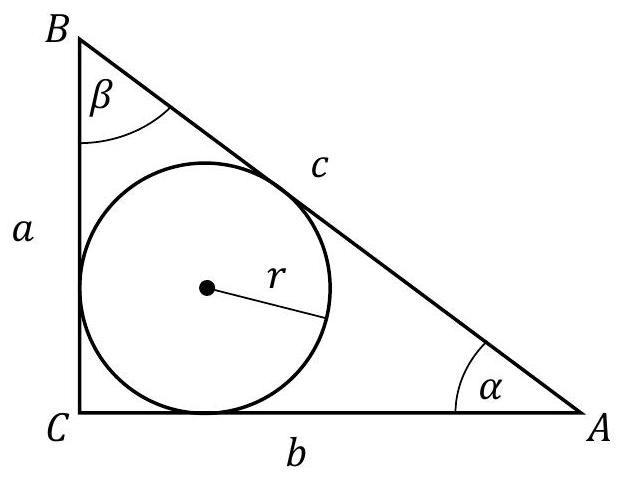
\includegraphics[max width=\textwidth, center]{2025_02_07_36131546116d12814c9cg-39}

Wtedy $a^{2}+b^{2}=c^{2}$ oraz $r=\frac{a+b-c}{2}$.\\
Z warunków zadania wynika, że $r=\frac{1}{5} c$.\\
Zatem

$$
\begin{gathered}
\frac{c}{5}=\frac{a+b-c}{2} \\
2 c=5 a+5 b-5 c \\
b=\frac{7}{5} c-a
\end{gathered}
$$

Podstawiając otrzymaną zależność do równości wynikającej z twierdzenia Pitagorasa, otrzymujemy:

$$
\begin{gathered}
a^{2}+\left(\frac{7}{5} c-a\right)^{2}=c^{2} \\
2 a^{2}-\frac{14}{5} a c+\frac{24}{25} c^{2}=0 \\
25 a^{2}-35 a c+12 c^{2}=0
\end{gathered}
$$

Potraktujmy otrzymane równanie jak równanie kwadratowe z niewiadomą a i parametrem c. Otrzymujemy zatem

$$
\begin{gathered}
\Delta=(-35 c)^{2}-4 \cdot 25 \cdot 12 c^{2}=25 c^{2} \\
a=\frac{35 c-5 c}{50}=\frac{3}{5} c \quad \text { lub } a=\frac{35 c+5 c}{50}=\frac{4}{5} c
\end{gathered}
$$

Gdy $a=\frac{3}{5} c$, to wtedy $b=\frac{7}{5} c-\frac{3}{5} c=\frac{4}{5} c$, a gdy $a=\frac{4}{5} c$, to $b=\frac{7}{5} c-\frac{4}{5} c=\frac{3}{5} c$. W każdym $z$ tych przypadków otrzymujemy więc taki sam trójkąt (z dokładnością do oznaczeń). Bez straty\\
ogólności można przyjąć, że $a=\frac{3}{5} c$ i $b=\frac{4}{5} c$. Przy oznaczeniach z rysunku mamy $\sin \alpha=\frac{a}{c}=\frac{\frac{3}{5} c}{c}=\frac{3}{5}$ oraz $\sin \beta=\frac{b}{c}=\frac{\frac{4}{5} c}{c}=\frac{4}{5}$. Kąty $\alpha$ i $\beta$ są ostre, więc ten z nich ma większą miarę, dla którego sinus przyjmuje większą wartość.\\
Zatem sinus większego z kątów ostrych trójkąta $A B C$ jest równy $\frac{4}{5}$.

\section*{Uwaga:}
Równanie $25 a^{2}-35 a c+12 c^{2}=0$ możemy też podzielić stronami przez $c^{2}$. Otrzymujemy wtedy równanie kwadratowe $25\left(\frac{a}{c}\right)^{2}-35 \cdot\left(\frac{a}{c}\right)+12=0$ z niewiadomą $\frac{a}{c}$. Rozwiązując to równanie, otrzymujemy $\frac{a}{c}=\frac{3}{5}$ lub $\frac{a}{c}=\frac{4}{5}$. Są to wartości sinusa kąta $\alpha$.

\section*{Sposób 2. (równość odcinków stycznych oraz twierdzenie Pitagorasa).}
Przyjmijmy następujące oznaczenia:\\
$a, b, c$-długości boków trójkąta $A B C$\\
$\alpha, \beta$ - miary kątów ostrych trójkąta\\
$r$ - promień okręgu wpisanego w trójkąt $A B C$. (Zobacz rysunek).\\
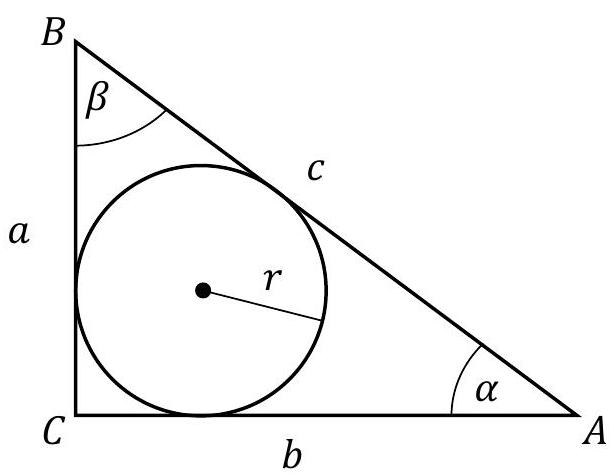
\includegraphics[max width=\textwidth, center]{2025_02_07_36131546116d12814c9cg-40}

Zakładamy, że bok $B C$ jest sumą odcinków o długościach $a-r$ oraz $r$.\\
Ponieważ z treści zadania wynika, że $c=5 r$, więc na mocy równości odcinków stycznych, przeciwprostokątna jest sumą odcinków o długościach $a-r$ oraz $5 r-(a-r)=6 r-a$. Otrzymujemy zatem trójkąt prostokątny $A B C$, którego boki mają długości: $a, 7 r-a$ oraz $5 r$. Stosujemy twierdzenie Pitagorasa i zapisujemy równanie z dwiema niewiadomymi:

$$
a^{2}+(7 r-a)^{2}=(5 r)^{2}
$$

To równanie jest równoważne równaniu $a^{2}-7 a r+12 r^{2}=0$.\\
Powyższe równanie traktujemy jako równanie kwadratowe z niewiadomą a iz parametrem $r$. Obliczamy wyróżnik:

$$
\Delta=(-7 r)^{2}-4 \cdot 1 \cdot 12 r^{2}=r^{2}
$$

i otrzymujemy dwa rozwiązania:

$$
a=\frac{7 r+r}{2}=4 r \text { oraz } a=\frac{7 r-r}{2}=3 r
$$

Jeśli $a=4 r$, to wtedy $b=7 r-4 r=3 r$. Jeśli $a=3 r$, to $b=7 r-3 r=4 r$.

W każdym z tych przypadków otrzymujemy więc taki sam trójkąt (z dokładnością do oznaczeń). Bez straty ogólności można przyjąć, że $a=4 r$ i $b=3 r$.\\
Przy oznaczeniach z rysunku mamy $\sin \alpha=\frac{a}{c}=\frac{4 r}{5 r}=\frac{4}{5}$ oraz $\sin \beta=\frac{b}{c}=\frac{3 r}{5 r}=\frac{3}{5}$. Ponieważ kąty $\alpha$ i $\beta$ są ostre, więc ten z nich ma większą miarę, którego sinus przyjmuje większą wartość.\\
Zatem sinus większego z kątów ostrych trójkąta $A B C$ jest równy $\frac{4}{5}$.

\section*{Sposób 3.}
Przyjmijmy następujące oznaczenia:\\
$a, b, c$-długości boków trójkąta $A B C$\\
$\alpha, \beta$ - miary kątów ostrych trójkąta\\
$r$ - promień okręgu wpisanego w trójkąt $A B C$. (Zobacz rysunek).\\
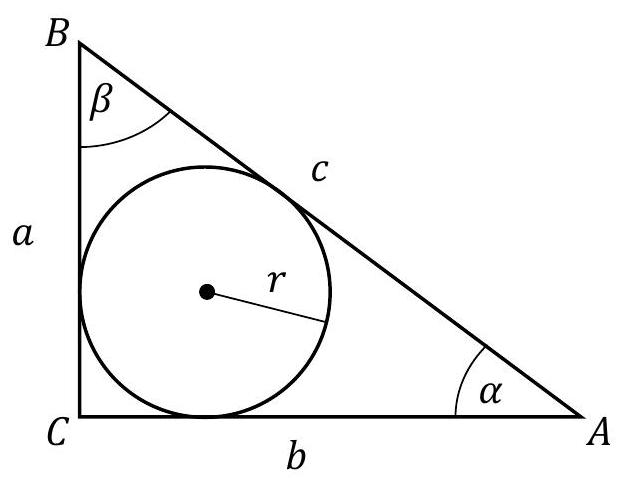
\includegraphics[max width=\textwidth, center]{2025_02_07_36131546116d12814c9cg-41}

Wtedy $a^{2}+b^{2}=c^{2}$ oraz $r=\frac{a+b-c}{2}$. $Z$ warunków zadania wynika, że $r=\frac{1}{5} c$. Zatem

$$
\begin{gathered}
\frac{c}{5}=\frac{a+b-c}{2} \\
2 c=5 a+5 b-5 c \\
5 a+5 b=7 c \\
\frac{a}{c}+\frac{b}{c}=\frac{7}{5}
\end{gathered}
$$

Ponieważ $\frac{a}{c}=\sin \alpha$ i $\quad \frac{b}{c}=\cos \alpha$, więc możemy zapisać równanie trygonometryczne

$$
\sin \alpha+\cos \alpha=\frac{7}{5}
$$

Z układu równań

$$
\left\{\begin{array}{l}
\sin \alpha+\cos \alpha=\frac{7}{5} \\
\sin ^{2} \alpha+\cos ^{2} \alpha=1
\end{array}\right.
$$

obliczamy $\sin \alpha=\frac{3}{5}$ lub $\sin \alpha=\frac{4}{5}$. Wówczas - odpowiednio do otrzymanych wartości $\sin \alpha$ - mamy: $\cos \alpha=\frac{4}{5}=\sin \beta$ lub $\cos \alpha=\frac{3}{5}=\sin \beta$.

Kąty $\alpha$ i $\beta$ są ostre, więc ten $z$ nich ma większą miarę, dla którego sinus przyjmuje większą wartość. Zatem sinus większego z kątów ostrych trójkąta $A B C$ jest równy $\frac{4}{5}$.

\section*{Sposób 4. (pole i obwód trójkata).}
Przyjmijmy następujące oznaczenia:\\
$a, b, c$ - długości boków trójkąta $A B C$\\
$\alpha, \beta$ - miary kątów ostrych trójkąta\\
$r$ - promień okręgu wpisanego w trójkąt $A B C$. (Zobacz rysunek).\\
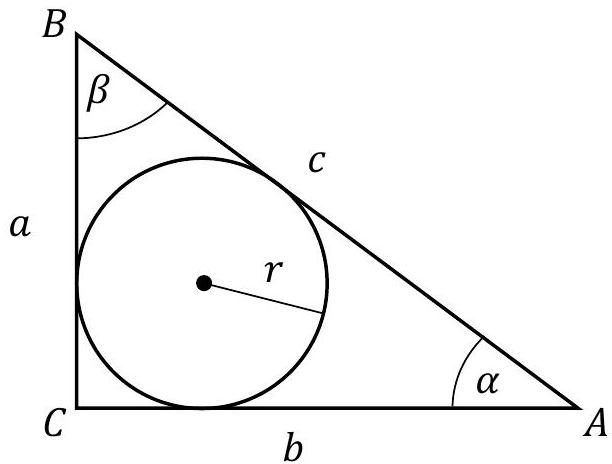
\includegraphics[max width=\textwidth, center]{2025_02_07_36131546116d12814c9cg-42}

Ponieważ z treści zadania wynika, że $c=5 r$, więc ze wzoru na promień okręgu wpisanego w ten trójkąt otrzymujemy zależność

$$
r=\frac{a+b-5 r}{2}
$$

Zatem

$$
a+b=7 r
$$

Ponadto wiemy, że pole trójkąta jest równe iloczynowi promienia okręgu wpisanego i połowy obwodu trójkąta, więc

$$
P_{\Delta}=r \cdot p=r \cdot \frac{1}{2}(a+b+c)=r \cdot \frac{1}{2}(7 r+5 r)=6 r^{2}
$$

Zapisujemy zatem układ równań

$$
\left\{\begin{array}{l}
\frac{1}{2} \cdot a \cdot b=6 r^{2} \\
a+b=7 r
\end{array}\right.
$$

Ponieważ $b=7 r-a$, więc pierwsze równanie przyjmuje postać $a \cdot(7 r-a)=12 r^{2}$. Po przekształceniach otrzymujemy równoważne równanie kwadratowe, w którym możemy przyjąć, że niewiadomą jest $a$, natomiast parametrem $r$ :

$$
-a^{2}+7 a r-12 r^{2}=0
$$

Obliczamy wyróżnik trójmianu stojącego po lewej stronie równania:

$$
\Delta=(7 r)^{2}-4 \cdot(-1) \cdot\left(-12 r^{2}\right)=r^{2}
$$

i otrzymujemy dwa rozwiązania:

$$
a=\frac{-7 r+r}{-2}=3 r \text { oraz } a=\frac{-7 r-r}{-2}=4 r
$$

Jeśli $a=3 r$, to wtedy $b=7 r-3 r=4 r$. Jeśli $a=4 r$, to $b=7 r-4 r=3 r$.\\
W każdym ztych przypadków otrzymujemy więc taki sam trójkąt (z dokładnością do oznaczeń). Bez straty ogólności można przyjąć, że $a=3 r$ i $b=4 r$.\\
Przy oznaczeniach z rysunku mamy $\sin \alpha=\frac{a}{c}=\frac{3 r}{5 r}=\frac{3}{5}$ oraz $\sin \beta=\frac{b}{c}=\frac{4 r}{5 r}=\frac{4}{5}$. Ponieważ kąty $\alpha$ i $\beta$ są ostre, więc ten z nich ma większą miarę, którego sinus przyjmuje większą wartość.\\
Zatem sinus większego z kątów ostrych trójkąta $A B C$ jest równy $\frac{4}{5}$.\\
Sposób 5.\\
Przyjmijmy następujące oznaczenia:\\
$S$ - środek okręgu wpisanego w trójkąt $A B C$\\
$D$ - punkt styczności okręgu wpisanego z prostą zawierającą przeciwprostokątną trójkąta\\
$a, b, c$-długości boków trójkąta $A B C$\\
$\alpha, \beta$ - miary kątów ostrych trójkąta\\
$r$ - promień okręgu wpisanego w trójkąt $A B C$. (Zobacz rysunek).\\
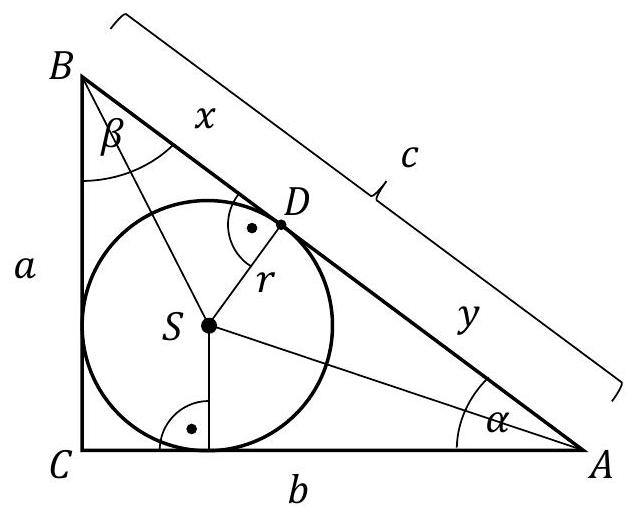
\includegraphics[max width=\textwidth, center]{2025_02_07_36131546116d12814c9cg-43}

Środek $S$ okręgu wpisanego w trójkąt jest punktem przecięcia dwusiecznych kątów wewnętrznych trójkąta. Zatem $|\Varangle D A S|=\frac{1}{2} \alpha$ i $|D B S|=\frac{1}{2} \beta$. Z definicji tangensa kąta ostrego otrzymujemy $\operatorname{tg} \frac{\alpha}{2}=\frac{r}{y}$ oraz $\operatorname{tg} \frac{\beta}{2}=\frac{r}{x}$. Stąd

$$
x=\frac{r}{\operatorname{tg} \frac{\beta}{2}} \quad \text { oraz } \quad y=\frac{r}{\operatorname{tg} \frac{\alpha}{2}}
$$

Z założenia wiemy, że $x+y=c=5 r$. Zatem

$$
\begin{gathered}
\frac{r}{\operatorname{tg} \frac{\beta}{2}}+\frac{r}{\operatorname{tg} \frac{\alpha}{2}}=5 r \\
\frac{1}{\operatorname{tg} \frac{\alpha}{2}}+\frac{1}{\operatorname{tg} \frac{\beta}{2}}=5
\end{gathered}
$$

Po uwzględnieniu zależności $\alpha+\beta=90^{\circ}$ otrzymujemy

$$
\frac{1}{\operatorname{tg}^{\frac{\alpha}{2}}}+\frac{1}{\operatorname{tg}\left(45^{\circ}-\frac{\alpha}{2}\right)}=5
$$

Stosujemy wzór na tangens różnicy kątów i przekształcamy otrzymane równanie

$$
\begin{gathered}
\frac{1}{\operatorname{tg} \frac{\alpha}{2}}+\frac{1+\operatorname{tg} 45^{\circ} \cdot \operatorname{tg} \frac{\alpha}{2}}{\operatorname{tg} 45^{\circ}-\operatorname{tg} \frac{\alpha}{2}}=5 \\
\frac{1}{\operatorname{tg} \frac{\alpha}{2}}+\frac{1+\operatorname{tg} \frac{\alpha}{2}}{1-\operatorname{tg} \frac{\alpha}{2}}=5 \\
1-\operatorname{tg} \frac{\alpha}{2}+\left(1+\operatorname{tg} \frac{\alpha}{2}\right) \cdot \operatorname{tg} \frac{\alpha}{2}=5\left(1-\operatorname{tg} \frac{\alpha}{2}\right) \cdot \operatorname{tg} \frac{\alpha}{2} \\
6\left(\operatorname{tg} \frac{\alpha}{2}\right)^{2}-5 \operatorname{tg} \frac{\alpha}{2}+1=0 \\
\left(2 \operatorname{tg} \frac{\alpha}{2}-1\right)\left(3 \operatorname{tg} \frac{\alpha}{2}-1\right)=0 \\
\operatorname{tg} \frac{\alpha}{2}=\frac{1}{2} \quad \text { lub } \quad \operatorname{tg} \frac{\alpha}{2}=\frac{1}{3}
\end{gathered}
$$

Gdy $\operatorname{tg} \frac{\alpha}{2}=\frac{1}{2}$, to wtedy $\operatorname{tg} \alpha=\frac{2 \operatorname{tg}\left(\frac{\alpha}{2}\right)}{1-\operatorname{tg}^{2}\left(\frac{\alpha}{2}\right)}=\frac{2 \cdot \frac{1}{2}}{1-\left(\frac{1}{2}\right)^{2}}=\frac{4}{3}$.\\
Gdy $\operatorname{tg} \frac{\alpha}{2}=\frac{1}{3}$, to wtedy $\operatorname{tg} \alpha=\frac{2 \operatorname{tg}\left(\frac{\alpha}{2}\right)}{1-\operatorname{tg}^{2}\left(\frac{\alpha}{2}\right)}=\frac{2 \cdot \frac{1}{3}}{1-\left(\frac{1}{3}\right)^{2}}=\frac{3}{4}$.\\
Zatem długości boków trójkąta mają się jak 3: 4:5 i sinus większego z kątów ostrych trójkąta jest równy $\frac{4}{5}$.

\section*{Sposób 6. (sinus podwojonego kata)}
Przyjmijmy następujące oznaczenia:\\
$a, b, c$-długości boków trójkąta $A B C$\\
$\alpha, \beta$ - miary kątów ostrych trójkąta\\
$r$ - promień okręgu wpisanego w trójkąt $A B C$. (Zobacz rysunek).\\
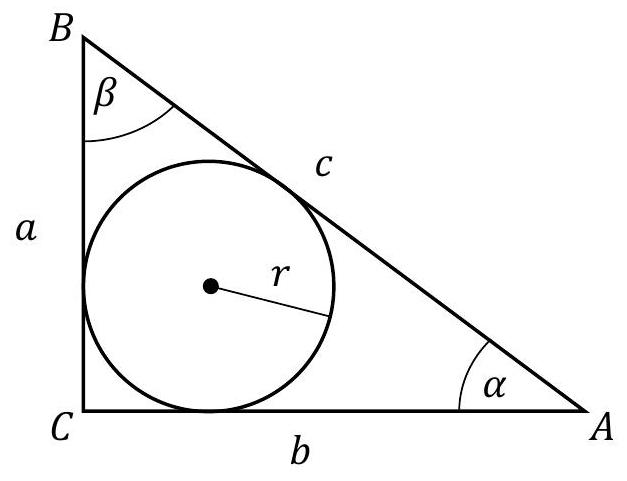
\includegraphics[max width=\textwidth, center]{2025_02_07_36131546116d12814c9cg-44}

Wtedy $r=\frac{a+b-c}{2}$. Z treści zadania wynika, że $c=5 r$.\\
Zatem

$$
\begin{gathered}
c=5 \cdot \frac{a+b-c}{2} \\
2 c=5 a+5 b-5 c \\
5 a+5 b=7 c
\end{gathered}
$$

Ponieważ obie strony tej równości są dodatnie, więc:

$$
\begin{gathered}
25 a^{2}+50 a b+25 b^{2}=49 c^{2} \\
25\left(a^{2}+b^{2}\right)+50 a b=49 c^{2} \\
25 c^{2}+50 a b=24 c^{2} \\
50 a b=24 c^{2}
\end{gathered}
$$

Ponieważ $a=c \cdot \sin \alpha$ oraz $b=c \cdot \cos \alpha$, więc powyższą równość możemy zapisać w postaci

$$
50 \cdot c^{2} \cdot \sin \alpha \cdot \cos \alpha=24 c^{2}
$$

a zatem

$$
25 \cdot \sin 2 \alpha=24
$$

czyli

$$
\sin 2 \alpha=\frac{24}{25}
$$

Korzystamy z tożsamości $\sin ^{2} 2 \alpha+\cos ^{2} 2 \alpha=1$ i otrzymujemy

$$
\cos ^{2} 2 \alpha=1-\left(\frac{24}{25}\right)^{2}=\frac{49}{625}
$$

Zatem $\cos 2 \alpha=\frac{7}{25}$ lub $\cos 2 \alpha=-\frac{7}{25}$. Ale $\cos 2 \alpha=1-2 \sin ^{2} \alpha$, więc

$$
1-2 \sin ^{2} \alpha=\frac{7}{25} \quad \text { lub } \quad 1-2 \sin ^{2} \alpha=-\frac{7}{25}
$$

Stąd

$$
\sin ^{2} \alpha=\frac{9}{25} \quad \text { lub } \quad \sin ^{2} \alpha=\frac{16}{25}
$$

Kąt $\alpha$ jest ostry, więc $\sin \alpha>0$. Zatem otrzymujemy $\sin \alpha=\frac{3}{5}$ lub $\sin \alpha=\frac{4}{5}$.\\
Wówczas - odpowiednio do otrzymanych wartości $\sin \alpha$-mamy: $\cos \alpha=\frac{4}{5}=\sin \beta$ lub $\cos \alpha=\frac{3}{5}=\sin \beta$. Ponieważ kątowi ostremu o większej mierze odpowiada większa wartość sinusa, więc sinus większego $z$ kątów ostrych trójkąta $A B C$ jest równy $\frac{4}{5}$.

Zadanie 14. (0-6)

\begin{center}
\begin{tabular}{|l|l|}
\hline
\multicolumn{2}{|c|}{Wymagania egzaminacyjne 2021} \\
\hline
\multicolumn{1}{|c|}{Wymaganie ogólne} & \multicolumn{1}{c|}{Wymagania szczegółowe} \\
\hline
III. Modelowanie matematyczne. & Zdający: \\
 & P4.9) wyznacza wzór funkcji kwadratowej \\
 & na podstawie pewnych informacji o tej \\
 & funkcji lub o jej wykresie; \\
 & R7.4) znajduje związki miarowe w figurach \\
 & płaskich [...]. \\
\hline
\end{tabular}
\end{center}

Łącznie za zadanie zdający może otrzymać 6 punktów: 3 punkty za rozwiązanie podpunktu a) oraz 3 punkty za rozwiązanie podpunktu b).

\section*{Zasady oceniania dla podpunktu a)}
\section*{Zdający otrzymuje}
gdy zapisze współrzędne punktu $C$ w zależności od zmiennej $m: C=\left(m, m^{2}\right)$.\\
Zdający otrzymuje ......................................................................................................... 2 p.\\
gdy:

\begin{itemize}
  \item wyznaczy wysokość $h_{C}$ trójkąta $A B C$ opuszczoną z wierzchołka $C$ w zależności od $m: h_{C}=\frac{\left|m-m^{2}+2\right|}{\sqrt{2}}$\\
ALBO
  \item wyznaczy współrzędne dwóch wektorów zaczepionych w jednym z wierzchołków trójkąta $A B C$, rozpinających trójkąt $A B C$, np. $\overrightarrow{A C}=\left[m, m^{2}-2\right], \overrightarrow{A B}=[1,1]$\\
ALBO
  \item wyznaczy długości odcinków $A C$ i $B C$ w zależności od zmiennej $m$ oraz wyznaczy długość odcinka $A B: \quad|A C|=\sqrt{m^{2}+\left(m^{2}-2\right)^{2}},|B C|=\sqrt{(m-1)^{2}+\left(m^{2}-3\right)^{2}}$, $|A B|=\sqrt{2}$
\end{itemize}

\section*{Zdający otrzymuje}
gdy zastosuje poprawną metodę i zapisze wzór na pole trójkąta $A B C$ w zależności od zmiennej $m$ :

$$
P(m)=\frac{1}{2} \cdot\left|m^{2}-m-2\right| \quad \text { dla } m \neq-1 \quad \text { i } \quad m \neq 2
$$

\section*{Uwagi:}
\begin{enumerate}
  \item Jeżeli zdający wyznaczy poprawny wzór funkcji $P(m)$, lecz nie poda dziedziny tej funkcji, to może za rozwiązanie podpunktu a) otrzymać 3 punkty.
  \item Jeżeli zdający przyjmuje $C=\left(x, x^{2}\right)$, konsekwentnie rozwiązuje podpunkt a) zadania do końca, otrzymując $P(x)=\frac{1}{2} \cdot\left|x^{2}-x-2\right|$, to może otrzymać co najwyżej 2 punkty.
\end{enumerate}

\section*{Zasady oceniania dla podpunktu b)}
Zdający otrzymuje 1 p. gdy:

\begin{itemize}
  \item zauważy, że trójkąt ten jest ostrokątny wtedy i tylko wtedy, gdy punkt $C$ leży na jednym z fragmentów $M_{1} M_{2}$ lub $N_{1} N_{2}$ paraboli\\
ALBO
  \item zapisze równania prostych prostopadłych do prostej $A B$ przechodzących przez punkt $A$ i $B$\\
ALBO
  \item zapisze, że w każdym z rozpatrywanych trójkątów $A B C$ kąt przy wierzchołku $C$ jest ostry i zapisze warunki na to, żeby kąty przy wierzchołkach $A$ i $B$ były ostre\\
ALBO
  \item zapisze warunki na to, aby kąty przy wierzchołkach $A, B$ i $C$ były ostre, np.: $\cos |\Varangle C A B|>0$ oraz $\cos |\Varangle A B C|>0$ oraz $\cos |\Varangle A C B|>0$\\
lub\\
$\cos |\Varangle(\overrightarrow{A B}, \overrightarrow{A C})|>0$ oraz $\cos |\Varangle(\overrightarrow{C A}, \overrightarrow{C B})|>0$ oraz $\cos |\Varangle(\overrightarrow{B A}, \overrightarrow{B C})|>0$\\
lub\\
$\overrightarrow{A B} \cdot \overrightarrow{A C}>0$ oraz $\overrightarrow{C A} \cdot \overrightarrow{C B}>0$ oraz $\overrightarrow{B A} \cdot \overrightarrow{B C}>0$\\
lub\\
$|A B|^{2}+|B C|^{2}>|C A|^{2},|B C|^{2}+|C A|^{2}>|A B|^{2},|A C|^{2}+|A B|^{2}>|B C|^{2}$\\
Zdający otrzymuje\\
gdy:
  \item wyznaczy równania prostych $M_{1} N_{1}$ oraz $M_{2} N_{2}$ oraz obliczy odcięte co najmniej dwóch punktów spośród $M_{1}, N_{1}, M_{2}, N_{2}$ i stwierdzi, że trójkąt ten jest ostrokątny wtedy i tylko wtedy, gdy punkt $C$ leży na jednym z fragmentów $M_{1} M_{2}$ lub $N_{1} N_{2}$ paraboli\\
ALBO
  \item zapisze układ nierówności:\\
i
\end{itemize}

$$
\begin{aligned}
& m^{2}+\left(m^{2}-2\right)^{2}+2-(m-1)^{2}-\left(m^{2}-3\right)^{2}>0 \\
& (m-1)^{2}+\left(m^{2}-3\right)^{2}+2-m^{2}-\left(m^{2}-2\right)^{2}>0 \\
& m^{2}+\left(m^{2}-2\right)^{2}+(m-1)^{2}+\left(m^{2}-3\right)^{2}-2>0
\end{aligned}
$$

ALBO

\begin{itemize}
  \item stwierdzi, że w każdym z rozpatrywanych trójkątów $A B C$ kąt przy wierzchołku $C$ jest ostry oraz zapisze układ nierówności:
\end{itemize}

$$
\begin{aligned}
& m^{2}+\left(m^{2}-2\right)^{2}+2-(m-1)^{2}-\left(m^{2}-3\right)^{2}>0 \\
& (m-1)^{2}+\left(m^{2}-3\right)^{2}+2-m^{2}-\left(m^{2}-2\right)^{2}>0
\end{aligned}
$$

i

ALBO

\begin{itemize}
  \item zapisze układ nierówności:
\end{itemize}

$$
m^{2}+m-2>0
$$

$$
m^{4}-4 m^{2}-m+6>0
$$

i

$$
-m^{2}-m+4>0
$$

\section*{Zdający otrzymuje}
gdy zastosuje poprawną metodę i wyznaczy wartości $m$ dla których trójkąt $A B C$ jest ostrokątny:\\
$m \in\left(\frac{-1-\sqrt{17}}{2},-2\right) \cup\left(1, \frac{-1+\sqrt{17}}{2}\right)$.

\section*{Uwaga:}
Jeżeli zdający, rozwiązując część b) sposobem 1., nie stwierdzi, że kąt przy wierzchołku $C$ jest zawsze ostry, to może otrzymać co najwyżej 2 punkty.

\section*{Przykładowe pełne rozwiązania}
\section*{a)}
\section*{Sposób 1.}
Niech $C$ będzie dowolnym punktem leżącym na paraboli. Wtedy $C=\left(m, m^{2}\right)$, gdzie $m$ jest dowolną liczbą rzeczywistą.\\
Długość odcinka $A B$ jest równa $|A B|=\sqrt{(1-0)^{2}+(3-2)^{2}}=\sqrt{2}$, a prosta $A B$ ma równanie postaci $y=x+2$, czyli $x-y+2=0$.\\
Wysokość $h_{C}$ trójkąta $A B C$ opuszczona z wierzchołka $C$ jest równa odległości punktu $C$ od prostej $A B$, więc ze wzoru na odległość punktu od prostej otrzymujemy

$$
h_{C}=\frac{\left|m-m^{2}+2\right|}{\sqrt{1^{2}+(-1)^{2}}}=\frac{\left|m-m^{2}+2\right|}{\sqrt{2}}
$$

Zatem pole $P$ trójkąta $A B C$ jest równe

$$
P=\frac{1}{2} \cdot|A B| \cdot h_{C}=\frac{1}{2} \cdot \sqrt{2} \cdot \frac{\left|m-m^{2}+2\right|}{\sqrt{2}}=\frac{1}{2} \cdot\left|m-m^{2}+2\right|
$$

dla $m \neq-1$ oraz $m \neq 2$ (gdy punkt $C$ leży na prostej $A B$, a więc gdy $m-m^{2}+2=0$, to trójkąt $A B C$ nie istnieje).

\section*{Sposób 2.}
Niech $C$ będzie dowolnym punktem leżącym na paraboli. Wtedy $C=\left(m, m^{2}\right)$, gdzie $m$ jest dowolną liczbą rzeczywistą. Wspórrzędne wektorów $\overrightarrow{A B}$ i $\overrightarrow{A C}$ są równe\\
$\overrightarrow{A B}=[1-0,3-2]=[1,1]$ oraz $\overrightarrow{A C}=\left[m-0, m^{2}-2\right]=\left[m, m^{2}-2\right]$\\
Zatem pole $P$ trójkąta $A B C$ jest równe

$$
P(m)=\frac{1}{2} \cdot\left|m \cdot 1-1 \cdot\left(m^{2}-2\right)\right|=\frac{1}{2} \cdot\left|m^{2}-m-2\right|
$$

dla $m \neq-1$ oraz $m \neq 2$ (gdy punkt $C$ leży na prostej $A B$, a więc gdy $m-m^{2}+2=0$, to trójkąt $A B C$ nie istnieje).\\
b)

\section*{Sposób 1.}
Zauważmy, że trójkąt $A B C$ jest ostrokątny wtedy i tylko wtedy, gdy punkt $C$ leży na jednym z fragmentów $M_{1} M_{2}$ lub $N_{1} N_{2}$ paraboli, gdzie końce tych fragmentów to punkty przecięcia prostych prostopadłych do prostej $A B$, przechodzących przez punkty $A$ i $B$, z parabolą (kąt przy wierzchołku $C$ tego trójkąta zawsze będzie kątem ostrym).\\
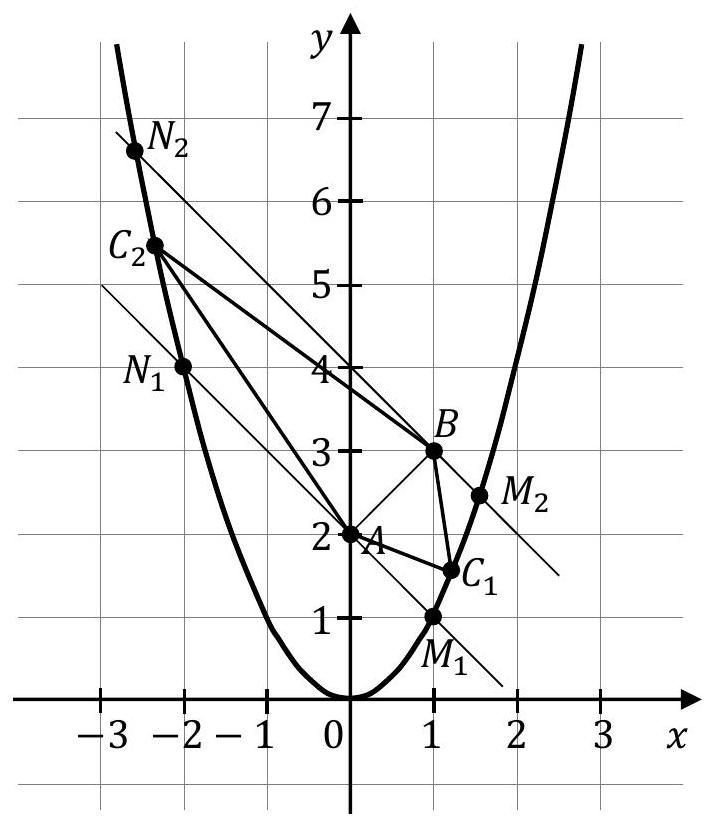
\includegraphics[max width=\textwidth, center]{2025_02_07_36131546116d12814c9cg-49}

Wystarczy w tym celu pokazać, że punkt $C$ nie leży w kole, którego średnicą jest odcinek $A B$. Promień tego koła jest równy $r=\frac{\sqrt{2}}{2}$, a środkiem koła jest punkt $S=\left(\frac{0+1}{2}, \frac{2+3}{2}\right)=\left(\frac{1}{2}, \frac{5}{2}\right)$, więc koło jest opisane nierównością

$$
\left(x-\frac{1}{2}\right)^{2}+\left(y-\frac{5}{2}\right)^{2} \leq \frac{1}{2}
$$

czyli

$$
\left(x-\frac{1}{2}\right)^{2}+\left(y-\frac{5}{2}\right)^{2}-\frac{1}{2} \leq 0
$$

Ponieważ

$$
\left(m-\frac{1}{2}\right)^{2}+\left(m^{2}-\frac{5}{2}\right)^{2}-\frac{1}{2}=m^{4}-4 m^{2}-m+6=\left(m^{2}-2,1\right)^{2}+0,2 m^{2}-m+1,59
$$

i wyróżnik trójmianu $0,2 m^{2}-m+1,59$ jest ujemny, więc

$$
\left(m-\frac{1}{2}\right)^{2}+\left(m^{2}-\frac{5}{2}\right)^{2}-\frac{1}{2}=\left(m^{2}-2,1\right)^{2}+0,2 m^{2}-m+1,59>0
$$

dla każdego $m \in R$.

To oznacza, że współrzędne punktu $C=\left(m, m^{2}\right)$ leżącego na paraboli, nie spełniają nierówności koła, czyli $C$ nie leży w kole, którego średnicą jest odcinek $A B$.

Współczynnik kierunkowy prostej $A B$ jest równy 1 , więc prosta prostopadła do $A B$ i przechodząca przez punkt $A$ ma równanie $y=-x+2$, natomiast prosta prostopadła do $A B$ i przechodząca przez punkt $B$ ma równanie $y=-x+4$.\\
Pierwsze współrzędne punktów $M_{1}$ i $N_{1}$ przecięcia prostej o równaniu $y=-x+2$ z parabolą obliczymy, rozwiązując równanie otrzymane z przyrównania prawych stron równań $y=-x+2$ i $y=x^{2}$. Otrzymujemy $x^{2}=-x+2$, więc $x_{M_{1}}=1$ oraz $x_{N_{1}}=-2$.\\
Podobnie obliczymy pierwsze współrzędne punktów $M_{2}$ i $N_{2}$. Po przyrównaniu prawych stron równań $y=-x+4$ i $y=x^{2}$ otrzymujemy $x^{2}=-x+4$, więc $x_{N_{2}}=\frac{-1-\sqrt{17}}{2}$ oraz $x_{M_{2}}=\frac{-1+\sqrt{17}}{2}$.\\
Zatem trójkąt $A B C$ jest ostrokątny tylko wtedy, gdy $m \in\left(\frac{-1-\sqrt{17}}{2},-2\right) \cup\left(1, \frac{-1+\sqrt{17}}{2}\right)$.

\section*{Uwagi:}
\begin{enumerate}
  \item Uzasadnienie, że punkt $C$ nie leży w kole o średnicy $A B$ można przeprowadzić też w następujący sposób. Promień tego koła jest równy $r=\frac{\sqrt{2}}{2}$, a środkiem tego koła jest punkt $S=\left(\frac{0+1}{2}, \frac{2+3}{2}\right)=\left(\frac{1}{2}, \frac{5}{2}\right)$. Rozważmy kwadrat opisany na tym kole, przy czym odcinek $A B$ łączy środki dwóch przeciwległych boków tego kwadratu. Wierzchołkami tego kwadratu są punkty $E=\left(\frac{1}{2}, \frac{3}{2}\right), F=\left(\frac{3}{2}, \frac{5}{2}\right), \quad G=\left(\frac{1}{2}, \frac{7}{2}\right), \quad H=\left(-\frac{1}{2}, \frac{5}{2}\right)$. Obszar ograniczony parabolą, w którym zawarty jest odcinek $A B$, jest opisany nierównością $y>x^{2}$. Ponieważ $\frac{3}{2}>\left(\frac{1}{2}\right)^{2}, \frac{5}{2}>\left(\frac{3}{2}\right)^{2}, \frac{7}{2}>\left(\frac{1}{2}\right)^{2}$ oraz $\frac{5}{2}>\left(-\frac{1}{2}\right)^{2}$, więc każdy z punktów $E, F, G$ i $H$ leży w tym obszarze. Obszar ten jest figurą wypukłą, więc kwadrat $E F G H$ jest zawarty w tym obszarze. Zatem koło wpisane w ten kwadrat również jest w tym obszarze zawarte. To oznacza, że żaden z punktów $C$ nie leży w kole o środku $S$ i średnicy $A B$.
  \item Uzasadnienie, że wyrażenie $m^{4}-4 m^{2}-m+6$ przyjmuje dla każdego $m \in R$ wartości dodatnie, można przeprowadzić też następująco. Gdy $m<2$, to wówczas $2-m>0$, więc $m^{4}-4 m^{2}-m+6=\left(m^{2}-2\right)^{2}+2-m>0$. Dla $m \geq 2$ mamy z kolei $m^{2}-2 \geq 2$, więc
\end{enumerate}

$$
\left(m^{2}-2\right)^{2}+2-m \geq 2\left(m^{2}-2\right)+2-m=2 m^{2}-m-2 \geq 2 \cdot 2^{2}-2-2>0
$$

\section*{Sposób 2.}
Aby wyznaczyć wszystkie wartości $m$, dla których trójkąt $A B C$ jest ostrokątny, wystarczy wyznaczyć te wartości $m$, dla których kąty $C A B, A B C$ i $A C B$ są ostre. Tak jest wtedy, gdy cosinusy tych kątów są dodatnie, czyli gdy

$$
\cos |\Varangle C A B|>0 \quad \text { i } \quad \cos |\Varangle A B C|>0 \quad \text { i } \cos |\Varangle A C B|>0 .
$$

Stąd iz twierdzenia cosinusów otrzymujemy

$$
\frac{b^{2}+c^{2}-a^{2}}{2 b c}>0 \quad \text { i } \quad \frac{a^{2}+c^{2}-b^{2}}{2 a c}>0 \quad \text { i } \quad \frac{b^{2}+a^{2}-c^{2}}{2 a b}>0
$$

gdzie $\quad a^{2}=|B C|^{2}=(m-1)^{2}+\left(m^{2}-3\right)^{2}, \quad b^{2}=|A C|^{2}=m^{2}+\left(m^{2}-2\right)^{2} \quad$ oraz $c^{2}=|A B|^{2}=2$.\\
Zatem

$$
b^{2}+c^{2}-a^{2}>0 \quad \text { i } \quad a^{2}+c^{2}-b^{2}>0 \quad \text { i } \quad b^{2}+a^{2}-c^{2}>0
$$

Rozwiązujemy pierwszą z tych nierówności:

$$
\begin{gathered}
b^{2}+c^{2}-a^{2}>0 \\
m^{2}+\left(m^{2}-2\right)^{2}+2-(m-1)^{2}-\left(m^{2}-3\right)^{2}>0 \\
2 m^{2}+2 m-4>0 \\
2(m-1)(m+2)>0 \\
m \in(-\infty,-2) \cup(1,+\infty)
\end{gathered}
$$

Rozwiązujemy drugą z nierówności:

$$
\begin{gathered}
a^{2}+c^{2}-b^{2}>0 \\
(m-1)^{2}+\left(m^{2}-3\right)^{2}+2-m^{2}-\left(m^{2}-2\right)^{2}>0 \\
-2 m^{2}-2 m+8>0 \\
\Delta=(-2)^{2}-4 \cdot(-2) \cdot 8=68 \\
m_{1}=\frac{2-\sqrt{68}}{-4}=\frac{-1+\sqrt{17}}{2}, \quad m_{2}=\frac{2+\sqrt{68}}{-4}=\frac{-1-\sqrt{17}}{2} \\
m \in\left(\frac{-1-\sqrt{17}}{2}, \frac{-1+\sqrt{17}}{2}\right)
\end{gathered}
$$

Nierówności $b^{2}+c^{2}-a^{2}>0$ i $a^{2}+c^{2}-b^{2}>0 \quad$ są spełnione jednocześnie dla $m \in\left(\frac{-1-\sqrt{17}}{2},-2\right) \cup\left(1, \frac{-1+\sqrt{17}}{2}\right)$.\\
Przekształcamy nierówność $b^{2}+a^{2}-c^{2}>0$ i otrzymujemy

$$
\begin{gathered}
m^{2}+\left(m^{2}-2\right)^{2}+(m-1)^{2}+\left(m^{2}-3\right)^{2}-2>0 \\
2 m^{4}-8 m^{2}-2 m+12>0 \\
m^{4}-4 m^{2}-m+6>0
\end{gathered}
$$

Wykażemy, że dla każdego $m \in\left(\frac{-1-\sqrt{17}}{2},-2\right) \cup\left(1, \frac{-1+\sqrt{17}}{2}\right)$ nierówność ta jest prawdziwa.\\
Nierówność $m^{4}-4 m^{2}-m+6>0$ możemy zapisać w postaci

$$
\left(m^{2}-2\right)^{2}+2-m>0
$$

Dla $m<2$ nierówność jest prawdziwa, gdyż lewa strona nierówności jest dodatnia. Ponieważ $\frac{-1+\sqrt{17}}{2}<\frac{-1+5}{2}=2$, więc dla każdego $m \in\left(\frac{-1-\sqrt{17}}{2},-2\right) \cup\left(1, \frac{-1+\sqrt{17}}{2}\right)$ nierówność $m^{4}-4 m^{2}-m+6>0$ jest prawdziwa.\\
Stąd trójkąt $A B C$ jest ostrokątny tylko dla $m \in\left(\frac{-1-\sqrt{17}}{2},-2\right) \cup\left(1, \frac{-1+\sqrt{17}}{2}\right)$.

\section*{Zadanie 15. (0-7)}
\begin{center}
\begin{tabular}{|l|l|}
\hline
\multicolumn{2}{|c|}{Wymagania egzaminacyjne 2021} \\
\hline
\multicolumn{1}{|c|}{Wymaganie ogólne} & \multicolumn{1}{c|}{Wymaganie szczegółowe} \\
\hline
III. Modelowanie matematyczne. & Zdający: \\
 & R11.6) stosuje pochodne do rozwiązywania \\
 & zagadnień optymalizacyjnych. \\
\hline
\end{tabular}
\end{center}

\section*{Zasady oceniania}
Rozwiązanie zadania optymalizacyjnego składa się z trzech etapów:

\begin{itemize}
  \item zbudowanie modelu opisującego sytuację podaną w zadaniu
  \item zbadanie modelu i jego własności
  \item przeprowadzenie końcowych obliczeń.
\end{itemize}

Pierwszy etap składa się $z$ trzech kroków.\\
Krok pierwszy: przyjęcie jednego z wymiarów zbiornika ( $x$ - długość krawędzi podstawy zbiornika, $h$ - wysokość zbiornika) za zmienną badanej funkcji i obliczenie drugiego wymiaru zbiornika:

$$
h=\frac{144}{x^{2}}
$$

lub

$$
x=\sqrt{\frac{144}{h}}
$$

Krok drugi: zapisanie funkcji kosztu wykonania $f$ zbiornika za pomocą jednej zmiennej:

$$
f(x)=100 x^{2}+4 x \cdot \frac{144}{x^{2}} \cdot 75
$$

lub

$$
f(h)=100 \cdot \frac{144}{h}+4 \cdot \sqrt{\frac{144}{h}} \cdot h \cdot 75
$$

Krok trzeci: ustalenie dziedziny funkcji $f: D_{x}=[4,9]$ lub $D_{h}=\left[\frac{16}{9}, 9\right]$.

Drugi etap składa się z trzech kroków.\\
Krok pierwszy: wyznaczenie pochodnej funkcji $f$ :

$$
f^{\prime}(x)=200 x-\frac{43200}{x^{2}}=200\left(x-\frac{216}{x^{2}}\right)
$$

lub

$$
f^{\prime}(h)=-\frac{14400}{h^{2}}+\frac{1800}{\sqrt{h}}
$$

Krok drugi: zastosowanie warunku koniecznego istnienia ekstremum funkcji $f$ - obliczenie miejsc zerowych pochodnej: $x=6$ (lub $h=4$ )

Krok trzeci: zbadanie znaku pochodnej funkcji $f$ :\\
$f^{\prime}(x)>0$ dla $x \in(6,9)$,\\
$f^{\prime}(x)<0$ dla $x \in(4,6)$\\
lub\\
$f^{\prime}(h)>0$ dla $h \in(4,9)$,\\
$f^{\prime}(h)<0$ dla $h \in\left(\frac{16}{9}, 4\right)$\\
oraz wyznaczenie (z uzasadnieniem) wartości zmiennej $x$ (lub zmiennej $h$ ), dla której funkcja $f$ przyjmuje wartość najmniejszą, np.:\\
funkcja $f$ zmiennej $x$ (określona na przedziale $[4,9]$ ) jest malejąca w przedziale $[4,6]$ oraz rosnąca w przedziale $[6,9]$, więc w punkcie $x=6$ funkcja $f$ osiąga najmniejszą wartość.

\section*{LUB}
funkcja $f$ zmiennej $h$ (określona na przedziale $\left[\frac{16}{9}, 9\right]$ )jest malejąca w przedziale $\left[\frac{16}{9}, 4\right]$ oraz rosnąca w przedziale $[4,9]$, więc w punkcie $h=4$ funkcja $f$ osiąga najmniejszą wartość.

Za poprawne wykonanie każdego z tych kroków zdający otrzymuje 1 punkt, o ile poprzednie kroki też były wykonane poprawnie.

Etap trzeci polega na obliczeniu wymiarów zbiornika, przy których koszt wykonania zbiornika jest najmniejszy:\\
$x=6, h=4$.\\
Za poprawne wykonanie trzeciego etapu zdający otrzymuje 1 punkt.

\section*{Uwagi:}
\begin{enumerate}
  \item Badanie znaku pochodnej zdający może opisać w inny sposób, np. szkicując wykres funkcji, która w ten sam sposób jak pochodna zmienia znak.
  \item Za poprawne uzasadnienie, że rozważana funkcja posiada wartość najmniejszą dla wyznaczonej wartości $x$ (czy też $h$ ), przy której pochodna się zeruje, można uznać sytuacje, gdy zdający:\\
a) opisuje słownie lub graficznie (np. przy użyciu strzałek) monotoniczność funkcji $f$; LUB\\
b) zapisuje, że dla wyznaczonej wartości $x$ (czy też $h$ ) funkcja $f$ ma minimum lokalne i jest to jednocześnie jej najmniejsza wartość.\\
Jeżeli zdający nie przedstawi takiego uzasadnienia, to za II etap może otrzymać co najwyżej 2 punkty.
  \item Jeżeli zdający wyznacza metodą prób i błędów wymiary zbiornika, przy których koszt wykonania zbiornika będzie najmniejszy, to otrzymuje 0 punktów za II i III etap..
  \item Jeżeli zdający rozpatruje funkcję kosztów postaci $f(x)=a x^{2}+\frac{b}{x}$ (gdzie $a>0, b>0$ ), nie uwzględniając wszystkich ścian bocznych lub uwzględniając dwie podstawy, to może otrzymać co najwyżej 5 punktów za całe rozwiązanie (nie otrzymuje punktów za drugi krok pierwszego etapu oraz za trzeci etap).
  \item Jeżeli zdający rozpatruje funkcję pola zamiast funkcji kosztów, to może otrzymać co najwyżej 5 punktów za całe rozwiązanie (nie otrzymuje punktów za drugi krok pierwszego etapu oraz za trzeci etap). Jeżeli zdający rozpatruje funkcję pola postaci $f(x)=a x^{2}+\frac{b}{x}$ (gdzie $a>0, b>0$ ), nie uwzględniajac wszystkich ścian bocznych lub uwzględniając dwie podstawy, to może otrzymać co najwyżej 4 punkty za całe rozwiązanie (nie otrzymuje punktów za drugi krok pierwszego etapu, trzeci krok drugiego etapu oraz za trzeci etap).
  \item Jeżeli zdający uzasadnia istnienie najmniejszej wartości funkcji kosztów w zbiorze $R \backslash\{0\}$, to nie otrzymuje punktu za trzeci krok drugiego etapu.
\end{enumerate}

\section*{Przykładowe pełne rozwiązania}
\section*{Sposób 1.}
Przyjmujemy następujące oznaczenia:\\
$x$ - długość krawędzi podstawy zbiornika (w metrach),\\
$h$ - wysokość zbiornika (w metrach).\\
Pojemność zbiornika ma wynosić $144 \mathrm{~m}^{3}$, więc $144=x^{2} \cdot h$. Stąd $h=\frac{144}{x^{2}}$.\\
Koszt $f$ wykonania zbiornika jest równy $f=100 x^{2}+75 \cdot 4 x h$, więc

$$
f(x)=100 x^{2}+4 x \cdot \frac{144}{x^{2}} \cdot 75
$$

gdzie $x \in[4,9]$.\\
Obliczamy pochodną funkcji $f$ :

$$
f^{\prime}(x)=200 x-\frac{43200}{x^{2}}
$$

Miejscem zerowym pochodnej funkcji $f$ jest $x=6$.\\
Badamy monotoniczność funkcji $f$ :\\
$f^{\prime}(x)>0$ dla $x \in(6,9)$,\\
$f^{\prime}(x)<0$ dla $x \in(4,6)$.

\section*{Zatem}
funkcja $f$ jest malejąca w przedziale $x \in[4,6]$,\\
funkcja $f$ jest rosnąca w przedziale $x \in[6,9]$.\\
Stąd funkcja $f$ przyjmuje najmniejszą wartość dla argumentu 6 . Wtedy $h=4$.\\
Wymiary zbiornika dla którego koszt wykonania jest najmniejszy: $6 \mathrm{~m} \times 6 \mathrm{~m} \times 4 \mathrm{~m}$.

\section*{Sposób 2.}
Przyjmujemy następujące oznaczenia:\\
$x$ - długość krawędzi podstawy zbiornika (w metrach),\\
$h$ - wysokość zbiornika (w metrach).\\
Pojemność zbiornika ma wynosić $144 \mathrm{~m}^{3}$, więc $144=x^{2} \cdot h$. Stąd $x=\sqrt{\frac{144}{h}}$.\\
Koszt $f$ wykonania zbiornika jest równy $f=100 x^{2}+75 \cdot 4 x h$, więc

$$
f(h)=100 \cdot \frac{144}{h}+4 h \cdot \sqrt{\frac{144}{h}} \cdot 75
$$

gdzie $h \in\left[\frac{16}{9}, 9\right]$.\\
Obliczamy pochodną funkcji $f$ :

$$
f^{\prime}(h)=-\frac{14400}{h^{2}}+\frac{3600}{2 \sqrt{h}}=-\frac{14400}{h^{2}}+\frac{1800}{\sqrt{h}}
$$

Miejscem zerowym pochodnej funkcji $f$ jest $h=4$.\\
Badamy monotoniczność funkcji $f$ :\\
$f^{\prime}(h)>0$ dla $h \in(4,9)$,\\
$f^{\prime}(h)<0$ dla $h \in\left(\frac{16}{9}, 4\right)$.

\section*{Zatem}
funkcja $f$ jest malejąca w przedziale $h \in\left[\frac{16}{9}, 4\right]$,\\
funkcja $f$ jest rosnąca w przedziale $h \in[4,9]$.\\
Stąd funkcja $f$ przyjmuje najmniejszą wartość dla argumentu $h=4$. Wtedy $x=6$.\\
Wymiary zbiornika, dla których koszt wykonania jest najmniejszy: $6 \mathrm{~m} \times 6 \mathrm{~m} \times 4 \mathrm{~m}$.

\section*{Uwaga:}
Zdający może rozwiązywać zadanie sposobem - za pomocą nierówności między średnią arytmetyczną i geometryczną, np.:

$$
\begin{aligned}
& f(x)=100 x^{2}+4 x \cdot \frac{144}{x^{2}} \cdot 75=100 x^{2}+\frac{43200}{x} \\
& f(x)=100\left(x^{2}+\frac{432}{x}\right)=100\left(x^{2}+\frac{216}{x}+\frac{216}{x}\right) \\
& \frac{x^{2}+\frac{216}{x}+\frac{216}{x}}{3} \geq \sqrt[3]{x^{2} \cdot \frac{216}{x} \cdot \frac{216}{x}}=\sqrt[3]{6^{3} \cdot 6^{3}}=36
\end{aligned}
$$

Stąd $f(x) \geq 100 \cdot 3 \cdot 36$ i funkcja $f(x)$ osiąga wartość najmniejsza, gdy $x^{2}=\frac{216}{x}$, tj. dla $x=6$. Wtedy $h=4$.


\end{document}